\chapter{Physical Layer}\label{ch:Phsic}
In this chapter the physical description and basic concepts implemented through this report will be discussed. The following are the basic assumptions and technology used to design, simulate and analysis the results of this thesis. In each section a different element of the communication link will be discussed, ultimately from this understanding it is perused to investigate nonlinear noise and its fundamental role in the transmission link. 
\section{Emission, Detection and Modulation}
The components of a coherent optical communication system will be given a short description in this section. The basic components  for an optical communication system are the  \textit{laser}, \textit{modulator} and \textit{detector}. For a coherent system the modulation format is an important design parameter, as was mentioned in the introduction, noise effects affect in different ways a given modulation format. Each component plays a fundamental role in a optical system; the correct selection of this elements can improve the throughput and transmission distance of a link. First let us consider the emission source that enabled coherent communication due to its high phase coherence, the \textit{distributed feedback laser} (DFB) laser.  

\subsection{Light Emitting Source }

In the beginning, coherent optical communications  did not get as much attention as IM/DD systems, because in the 1990 all available  light sources presented large phase noise and frequency drift~\cite{kikuchi2010coherent}, which is not useful for a coherent system. With the invention of the DFB laser new interest sprung in coherent systems. The main advantage of a DFB laser is the ability to emit a single longitudinal mode, which implies high frequency and phase stability.
 
 
A DFB laser is either a semiconductor laser or fiber laser where its whole resonator consists of a periodic structure, that acts as a distributed reflector. This reflector can be designed to reflect the desired wavelength range, which is amplified in the gain medium and emitted by the laser~\cite{FundPhoto,DFBtunable}. The emitted optical spectrum for a general DFB laser is shown in Figure~\ref{fig:DFB}, where we can see that a single mode is prevalent over all other noise present.
The linewidth of a DFB laser is usually bellow 10~MHz~\cite{kikuchi2010coherent} and for this implementation a narrow linewidth laser was simulated with a 1MHz linewidth. Wavelength  tunability is also possible for a range of 1000~GHz or a wavelength range of 8~nm, allowing the implementation of WDM systems~\cite{kikuchi2010coherent,DFBtunable}. A critical advantage for coherent systems is the use of HOM, which increase the systems capacity for the same bandwidth. Thus, modulating a DFB laser and detecting its physical properties like intensity, amplitude and phase are necessary to achieve higher system capacity.   
 \begin{figure}[h]
  \centering
  \subfloat[Nyquist spectral shaping on 5 channels]{\label{fig:WDM}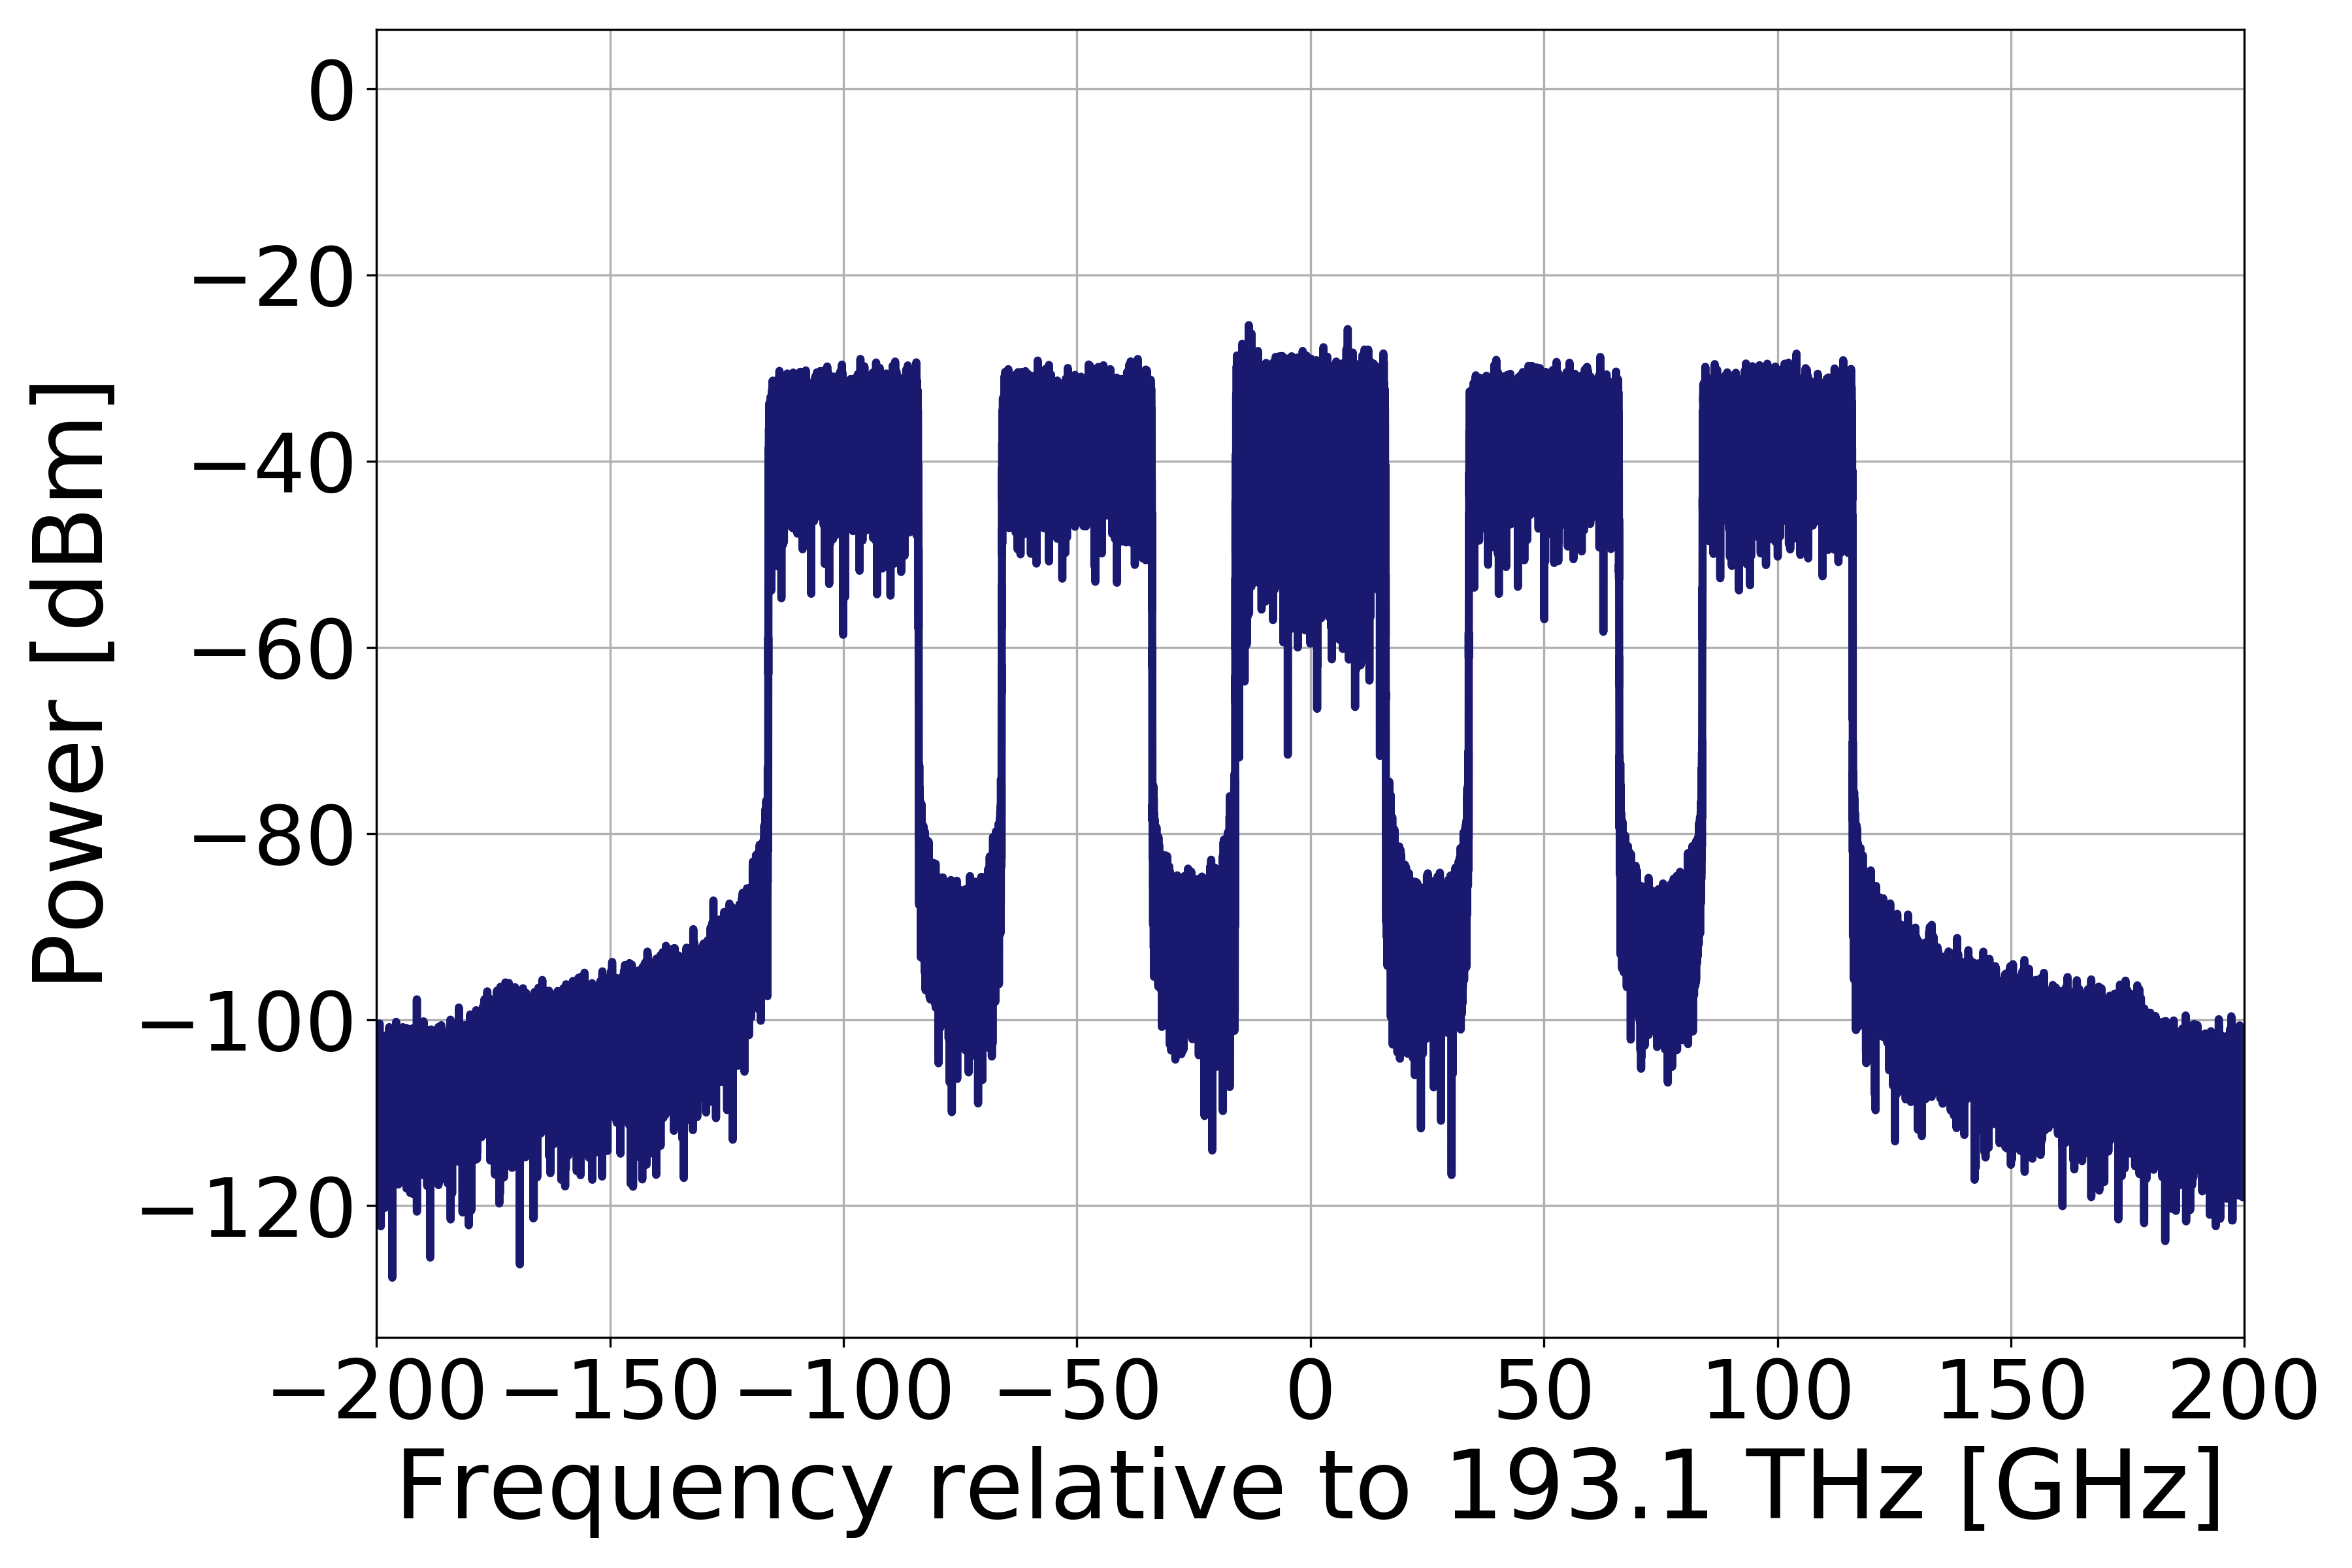
\includegraphics[width=.45\textwidth]{OPSDWM.png}}
  \qquad
  \subfloat[Single channel QAM modulation]{\label{fig:CHQAM}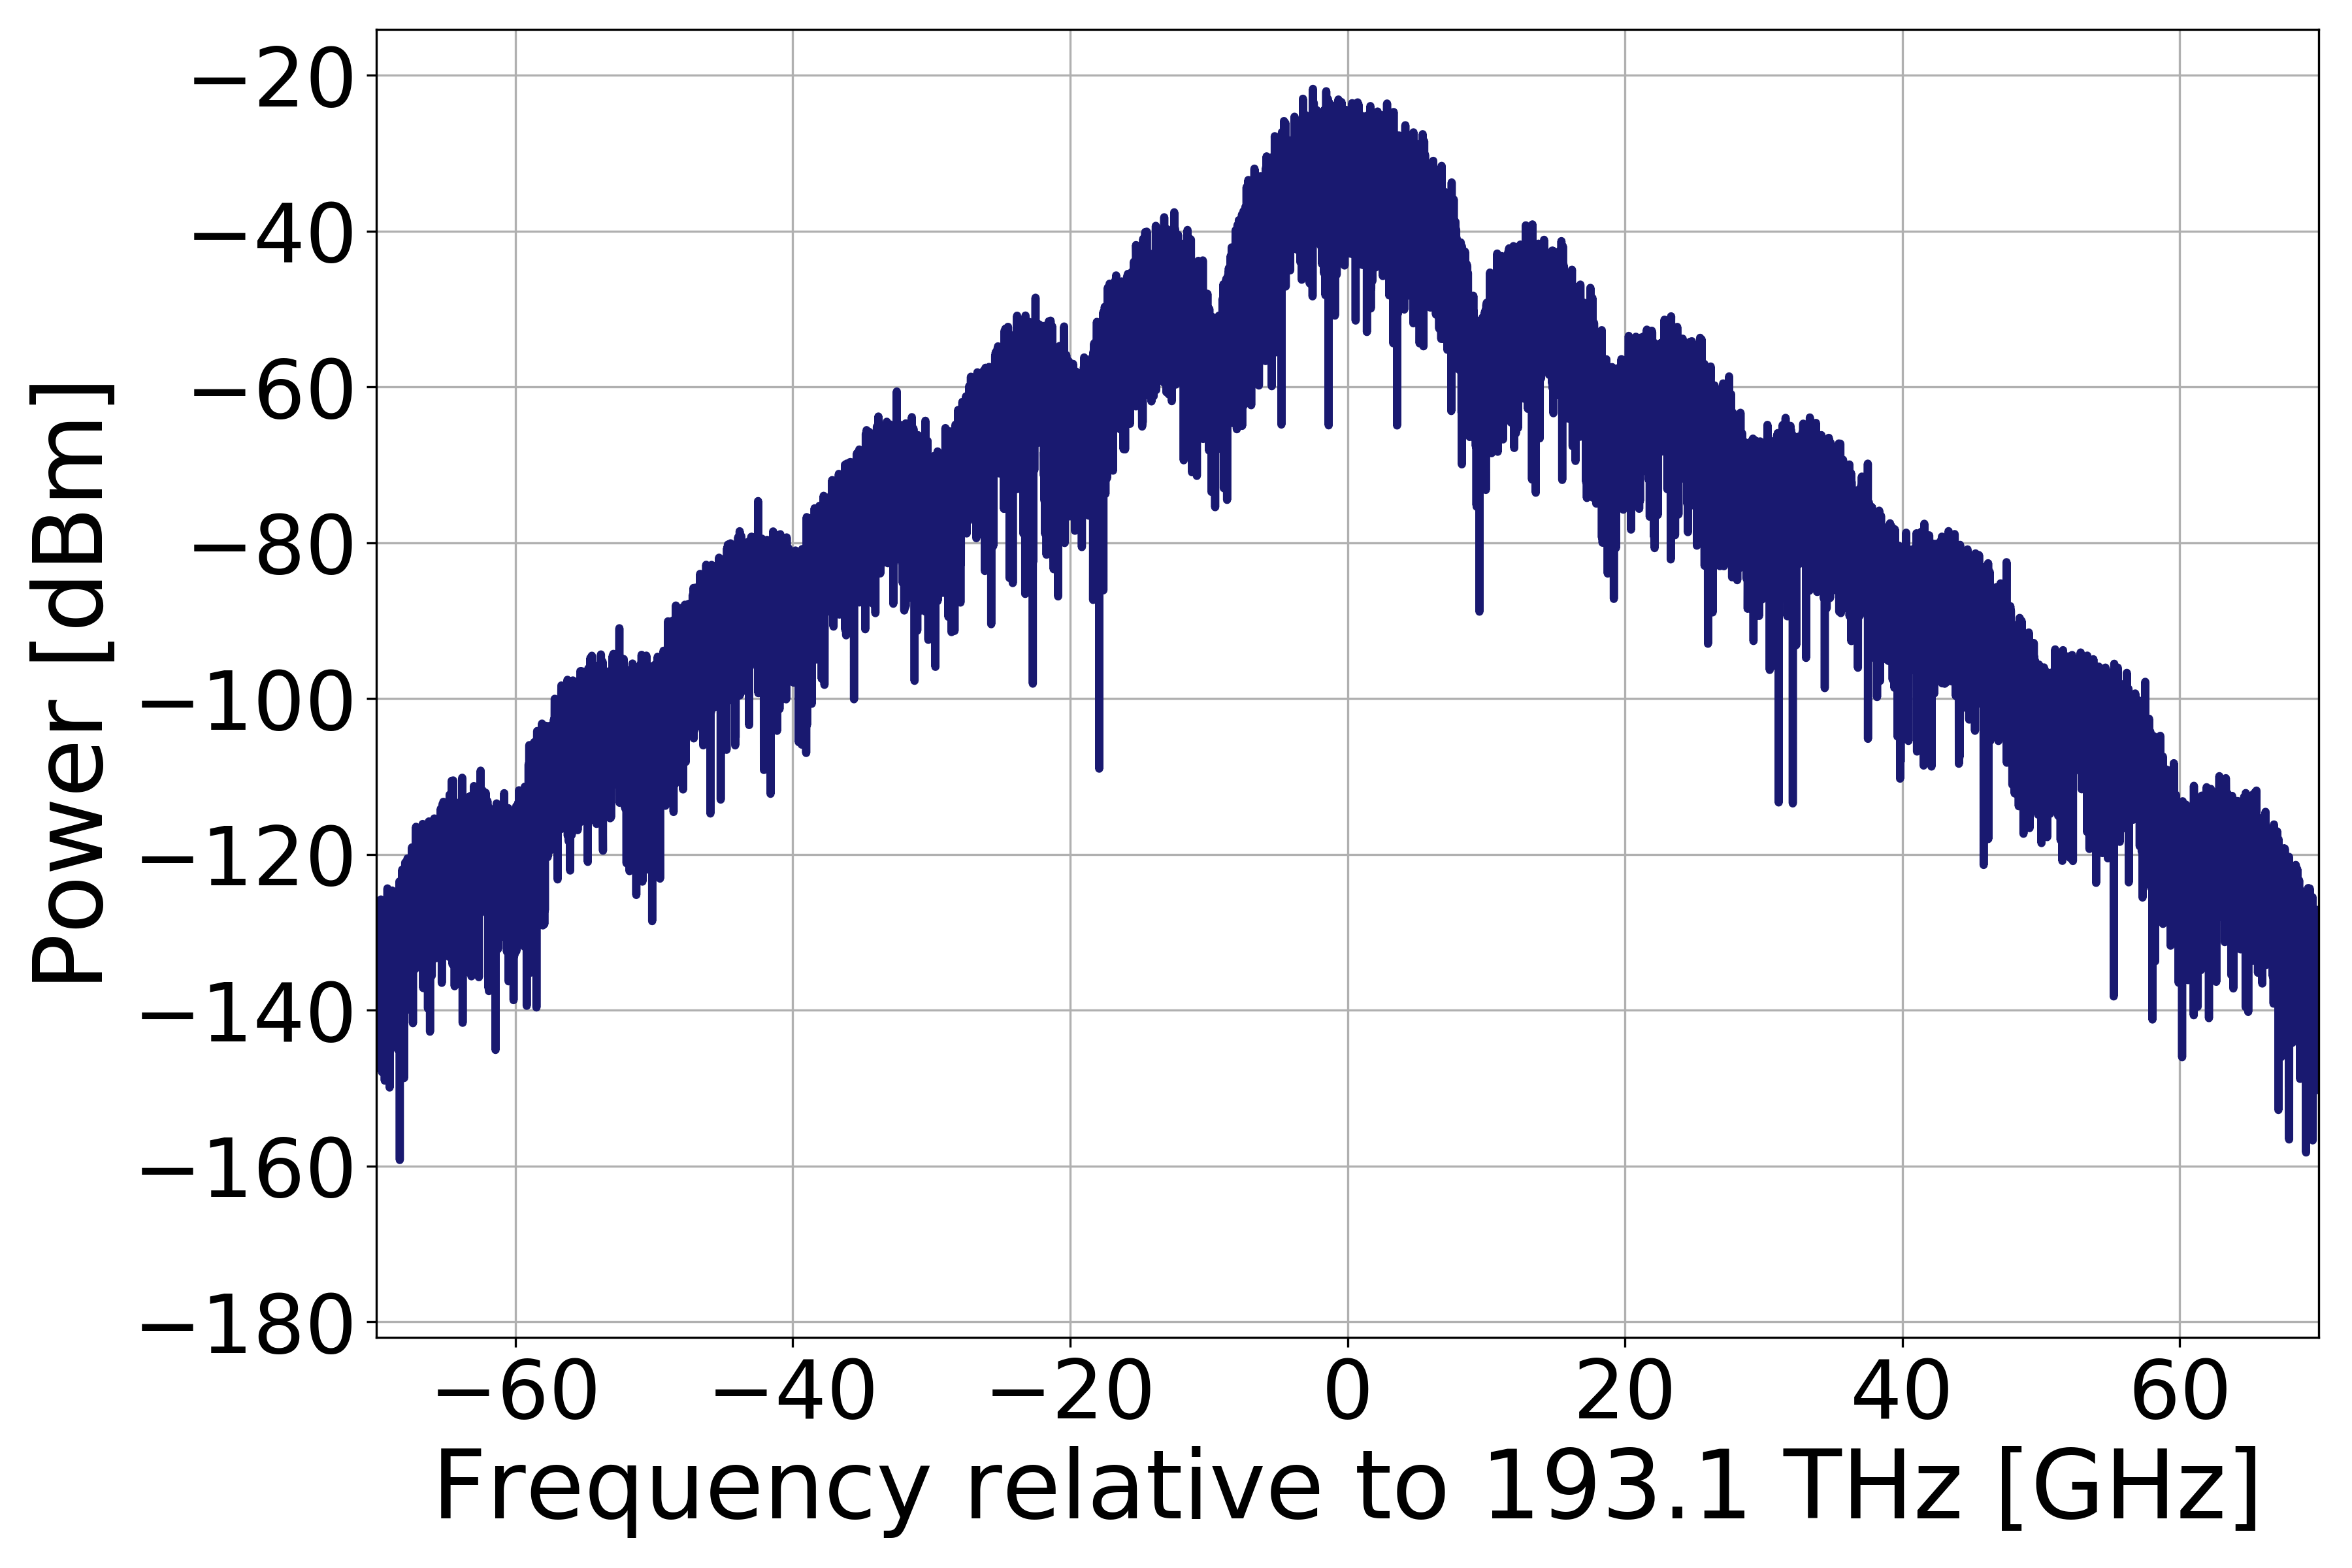
\includegraphics[width=.45\textwidth]{OPSQAM.png}} 
  \qquad
  \subfloat[No Modulation]{\label{fig:DFB}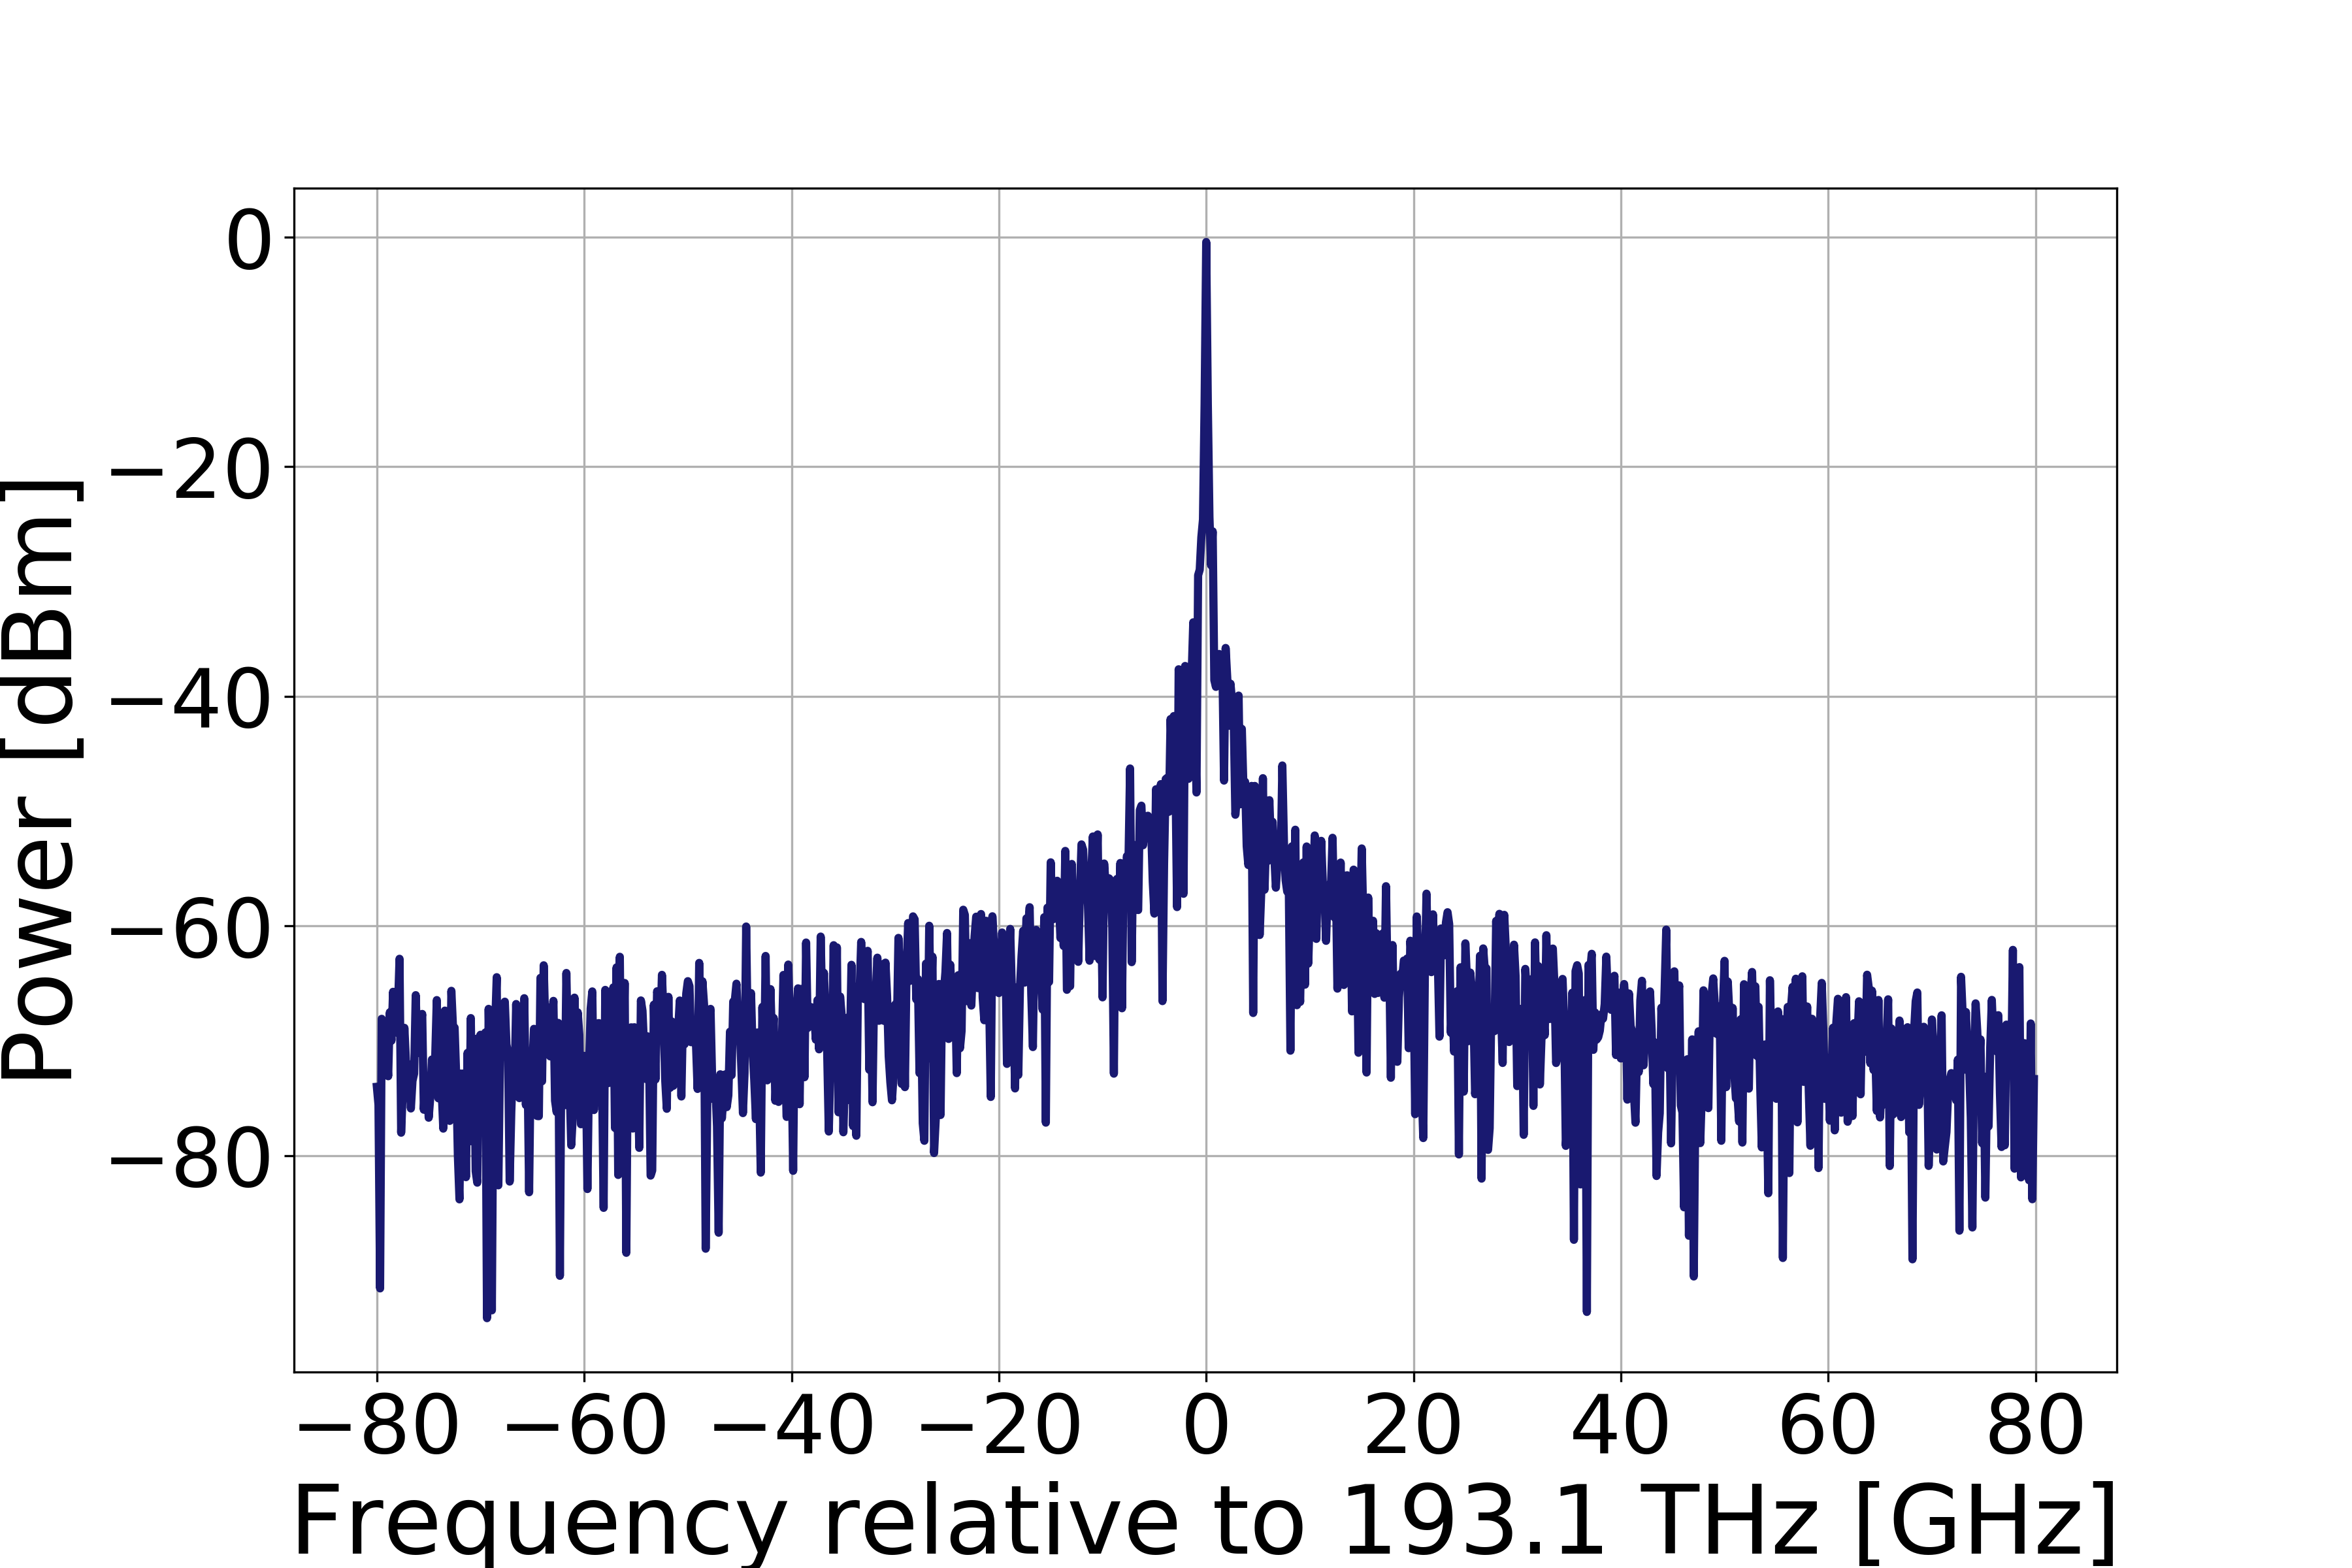
\includegraphics[width=0.45\textwidth]{OPS1mw.png}}     
  \caption{Optical frequency spectrum for different systems. A DFB laser frequency spectrum is shown in (c) and a set frequency spectrum after modulation are also shown in (a) and (b). }
  \label{fig:OpSpectrum}
\end{figure}

 To determine the operating power of a fiber system two noise sources constrain the system. The first noise source arises from the optical fibers refractive index dependence on the transmitted signal power~\cite{FiberAgrawal}. With a high power signal distortions can be induced if power fluctuations interact with the electrical susceptibility of the fiber. The second noise sources is common amplification effect when a low power signal is amplified AWGN noise is added~\cite{agrawal2001applications}, decreasing the OSNR and transmission length. Optical modulators require a strong carrier signal to operate at high OSNR. This requirements limits the minimum operating power. To determine the optimal operating range a detailed analysis will be discussed throughout this thesis.   


\subsection{Modulator and Detector}\label{sec:moddet}
Some of the advantages of optical communication systems rely on the modulation of the carrier signal and on the high sensitivity detection. To transmit more information over the same bandwidth a clever representation of the signal has to be standardized, as is done by HOM. However, it is necessary to modulate the carrier signal physical properties with precision to control reliably the information transmitted. Detection in coherent optical communication requires a scheme that can extract simultaneously multiple physical measurements from a single pulse. These two requirements can be solved with clever implementation and design of well understood optical phenomena.

In coherent communication the amplitude and phase of the carrier signal are modulated to transmit information. For an optical system \textit{phase modulation} (PM) can be achieved by passing through a non-centrosymmetric crystal that presents the Pockels effect~\cite{FiberAgrawal,kikuchi2015fundamentals}. This type of crystal have refractive index dependent on the applied voltage allowing PM~\cite{kikuchi2015fundamentals}. If a set of this crystals are used in a Mach-Zehnder configuration \textit{amplitude modulation} (AM) can be achieved.  This type of modulators are known as \textit{Mach-Zehnder-type push-pull modulators} or \textit{Mach-Zehnder modulator} (MZM)~\cite{kikuchi2015fundamentals}. To obtain a simultaneous amplitude and phase (In-phase and quadrature components)  modulation two MZM in parallel with a $\pi/2$ phase shift can be combined as shown in Figure~\ref{fig:DDMzm}, modulating independently the IO  components~\cite{kikuchi2015fundamentals}. Any kind of multilevel modulation format can be done with this scheme~\cite{ho2005generation},currently  integrated Dual-drive MZM LiNbO$_3$ IQ modulators are available on the market. This is the same modulator architecture that was used for the simulation.   


Modulation of the CW optical carrier not only alters the IQ components but it also modifies the optical spectrum of the laser. When  the optical carrier undergoes QAM, the optical spectrum of the transmitted signal is altered as seen in Figure~\ref{fig:CHQAM}. In Figure~\ref{fig:DetMod} the modulator is controlled  by the \textit{digital to analog converters } (DAC) and the driving signal is computed by \textit{digital signal processing} (DSP)~\cite{kikuchi2015fundamentals}. Filtering can be done by the DSP in the digital domain to modify the optical frequency spectrum of the signal and frequency spectrum close to a square pulse~\cite{kikuchi2015fundamentals,FiberAgrawal}, as seen in Figure~\ref{fig:WDM}. The type of filtering implemented is a low-pass filter with a transfer function response as a raised cosine function, aslo know as \textit{raised-cosine filter}. This type of filtering is known as Nyquist filtering and helps reduce the inter-symbol interference and maximize the available bandwidth~\cite{zou2016spectrally}, both of this effects can be observed in  Figure\ref{fig:WDM}. Reducing inter-symbol interference alludes to the clear spacing between channels, and maximizing the bandwidth can also be achieved given that each channel is constrained in a small bandwidth allowing more channels to be add in the side bands.

\begin{figure}[h!]
 \centering
\subfloat[Dual-drive MZM ]{\label{fig:DDMzm}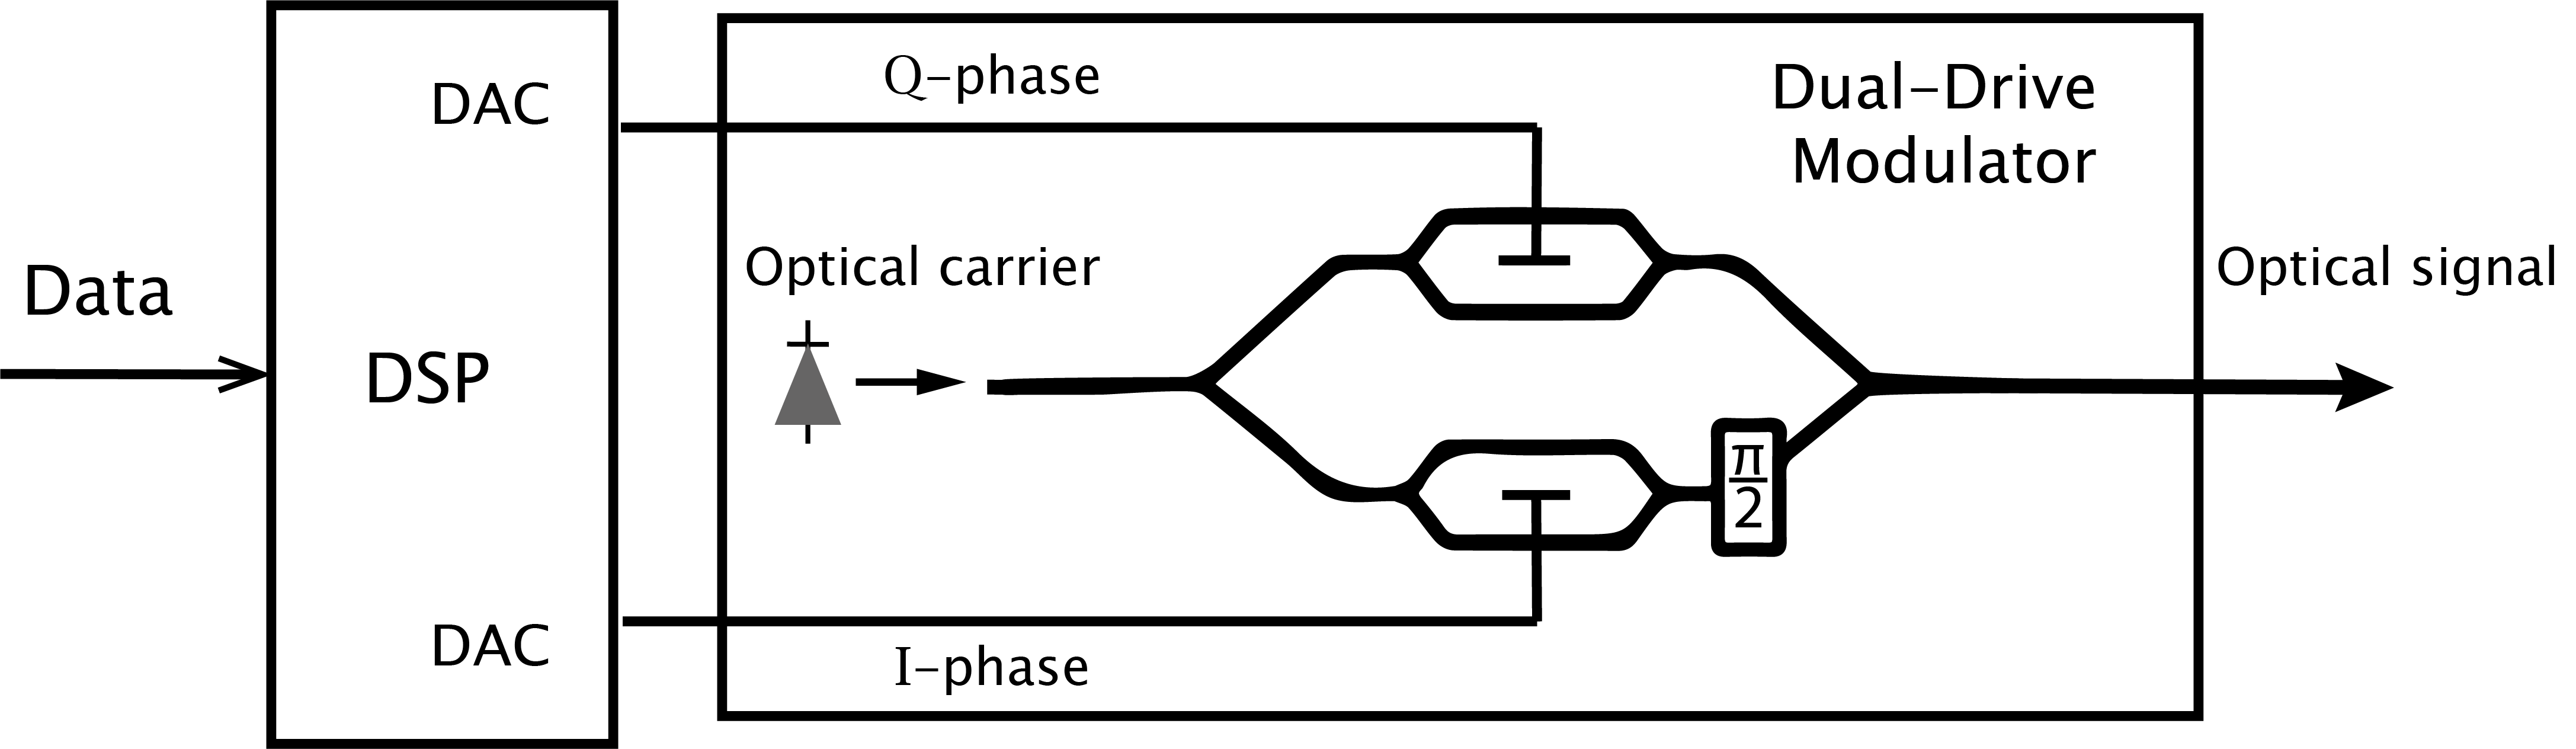
\includegraphics[width=\textwidth]{Dual-DriveModulator.png}}
  \qquad
  \subfloat[Phase-diversity homodyne reciver]{\label{fig:hOMODe}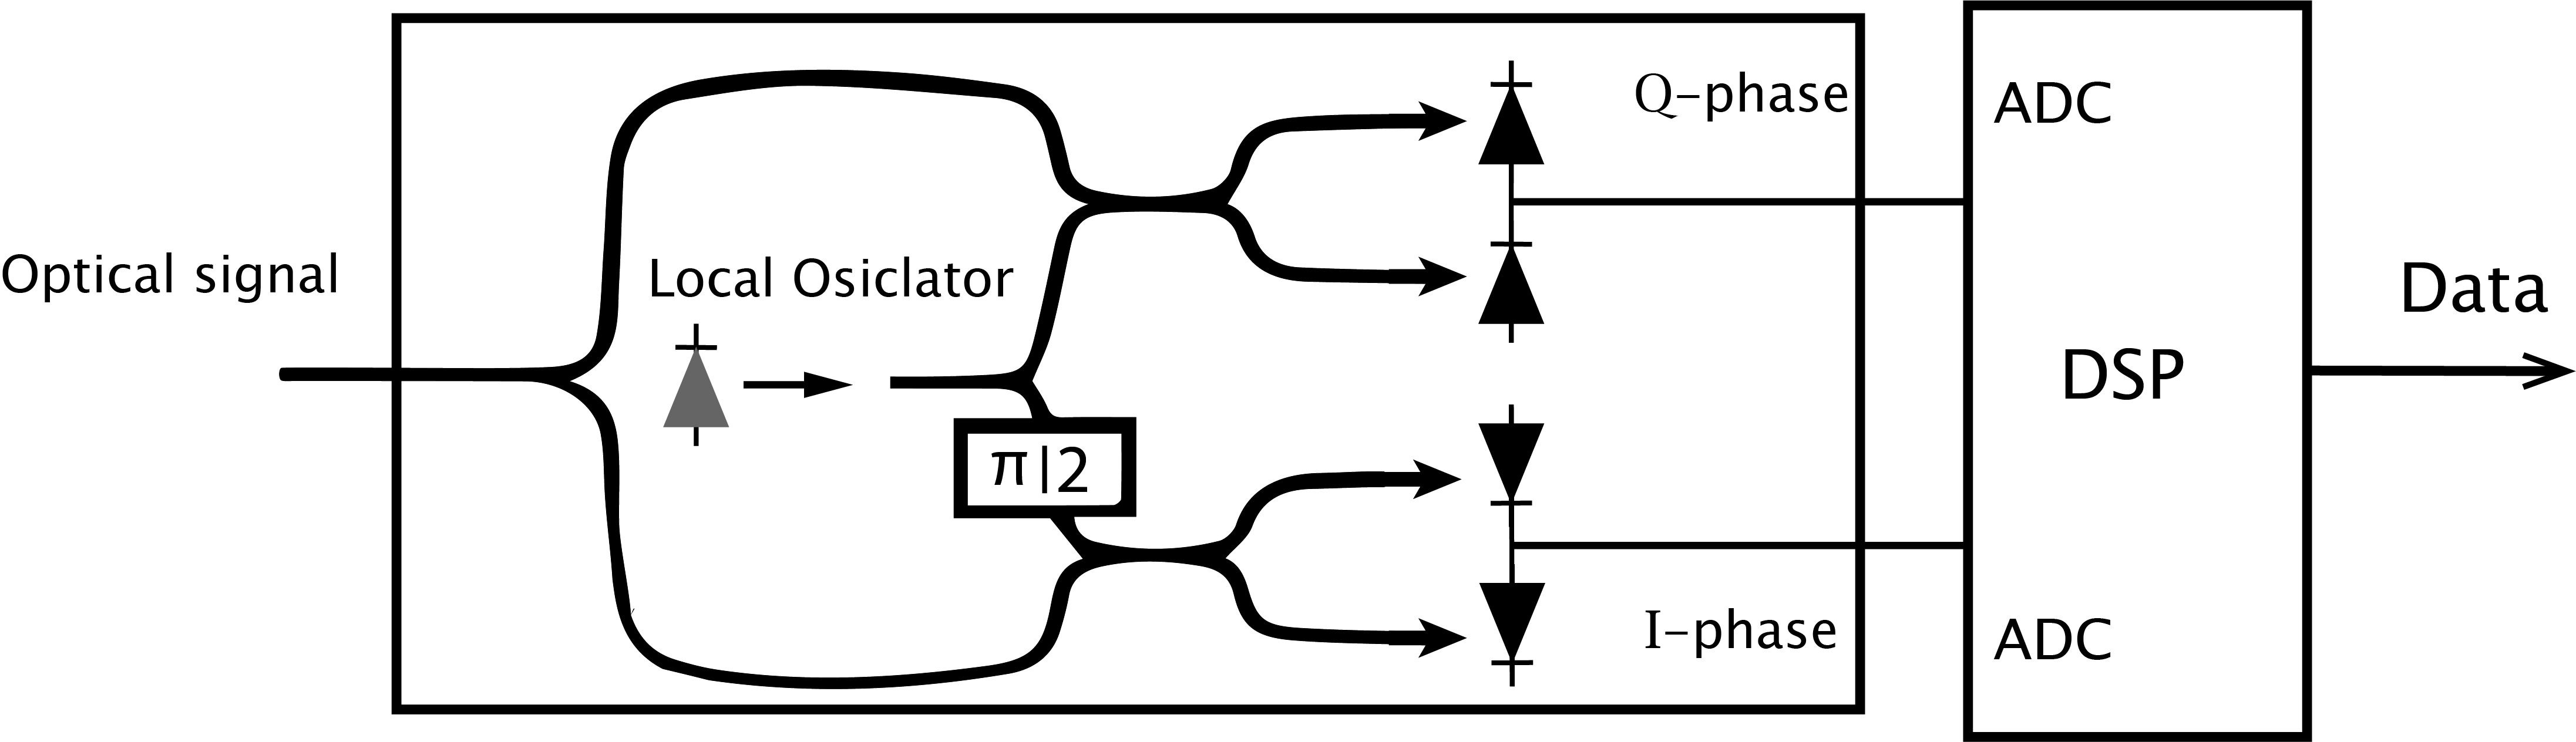
\includegraphics[width=\textwidth]{Hdetector.png}} 
  \caption{Detection and modulation scheme for a coherent optical communication system.\\ {\scriptsize Image designed inspired by available figures in Reference~\cite{ho2005generation,kikuchi2015fundamentals}} }
  \label{fig:DetMod}
\end{figure}


Coherent detection of the quadrature and in-phase components of the optical signal can be done simultaneously using a \textit{phase-diversity homodyne receiver}. The fundamental idea behind coherent detection is to compute the inner product of the \textit{local oscillator} (LO) phasor and the received signal phasor to determine one of the signals quadratures~\cite{kikuchi2015fundamentals}. A homodyne  receiver has LO operating at the same frequency as the carrier signal~\cite{FiberAgrawal}. However, to detect both IQ components simultaneously two LO signals are needed with a $\pi/2$ offset. This LO architecture, as shown in Figure~\ref{fig:hOMODe}, is called phase-diversity detection. Polarization diversity detection can be done with another LO that has orthogonal polarization, most commonly a random polarization state laser is used that is then divided using a polarization beam splitter~\cite{kikuchi2015fundamentals}. As for the modulator, an \textit{analog to digital conversion} (ADC) converts the signal to a digital sequence that can be processed by the DSP. Many different DSP schemes exist today to process an optical signal and retrieve the carriers phase~\cite{kuschnerov2009dsp}, determine the timing (clock recovery)~\cite{stojanovic2011clock}, LO offset mitigation ~\cite{kikuchi2015fundamentals,kuschnerov2009dsp} and other processing can be done to improve the signal quality.





\subsection{Modulation Format}

In the previous section, a short description of a dual-drive MZM was given. In this section,  the \textit{multi-level modulation} (or higher order modulation HOM) of the optical carrier will be discussed, which improves the link's spectral efficiency. In the digital domain the transmission of bits is mapped to a set of IQ components that determine the driving voltage of the modulator, producing the encoded optical signal that can be decoded on the receiver side. For the digital transmission, $m$ bits are collected and mapped to a complex symbol chosen from an alphabet
\begin{equation}
s(k)=i_{k}+jq_{k} \in \left\{s_{0},s_{1},...,s_{M-1}\right\},\ M=2^{m} 
\end{equation}
where k represents the symbols interval with length $T_{S}=mT_{B}$ and $1/T_{B}$ is the bit rate~\cite{seimetz2005multi}. One of the symbols in the alphabet is assigned depending on the bit combination, that is defined in a \textit{constellation diagram}, where $i$ and $q$ are the IQ component of each constellation point. When $m$ bit alphabet is designed, a $M$ point constellation is defined, the architecture of this constellation can follow a determined standard like PSK, QPSK or QAM (as discussed in Section~\ref{sec:modform}. In this project a  4 bit alphabet with a square 16QAM constellation was implemented as is shown in Figure~\ref{fig:16QAMcons}. A detailed explanation on how to determine the complex function that modulates the carrier signal and what electrical driving signal should sent the the MZM can be found in Reference~\cite{seimetz2005multi}. With this basic principals, our interest is shifted to the interaction between the transmitted optical signal and the optical fiber that guides the signal to the receiver. This interaction deteriorates the quality of the channel by corrupting the phase information imprinted by the modulators.   
 
\begin{figure}[h]
\centering
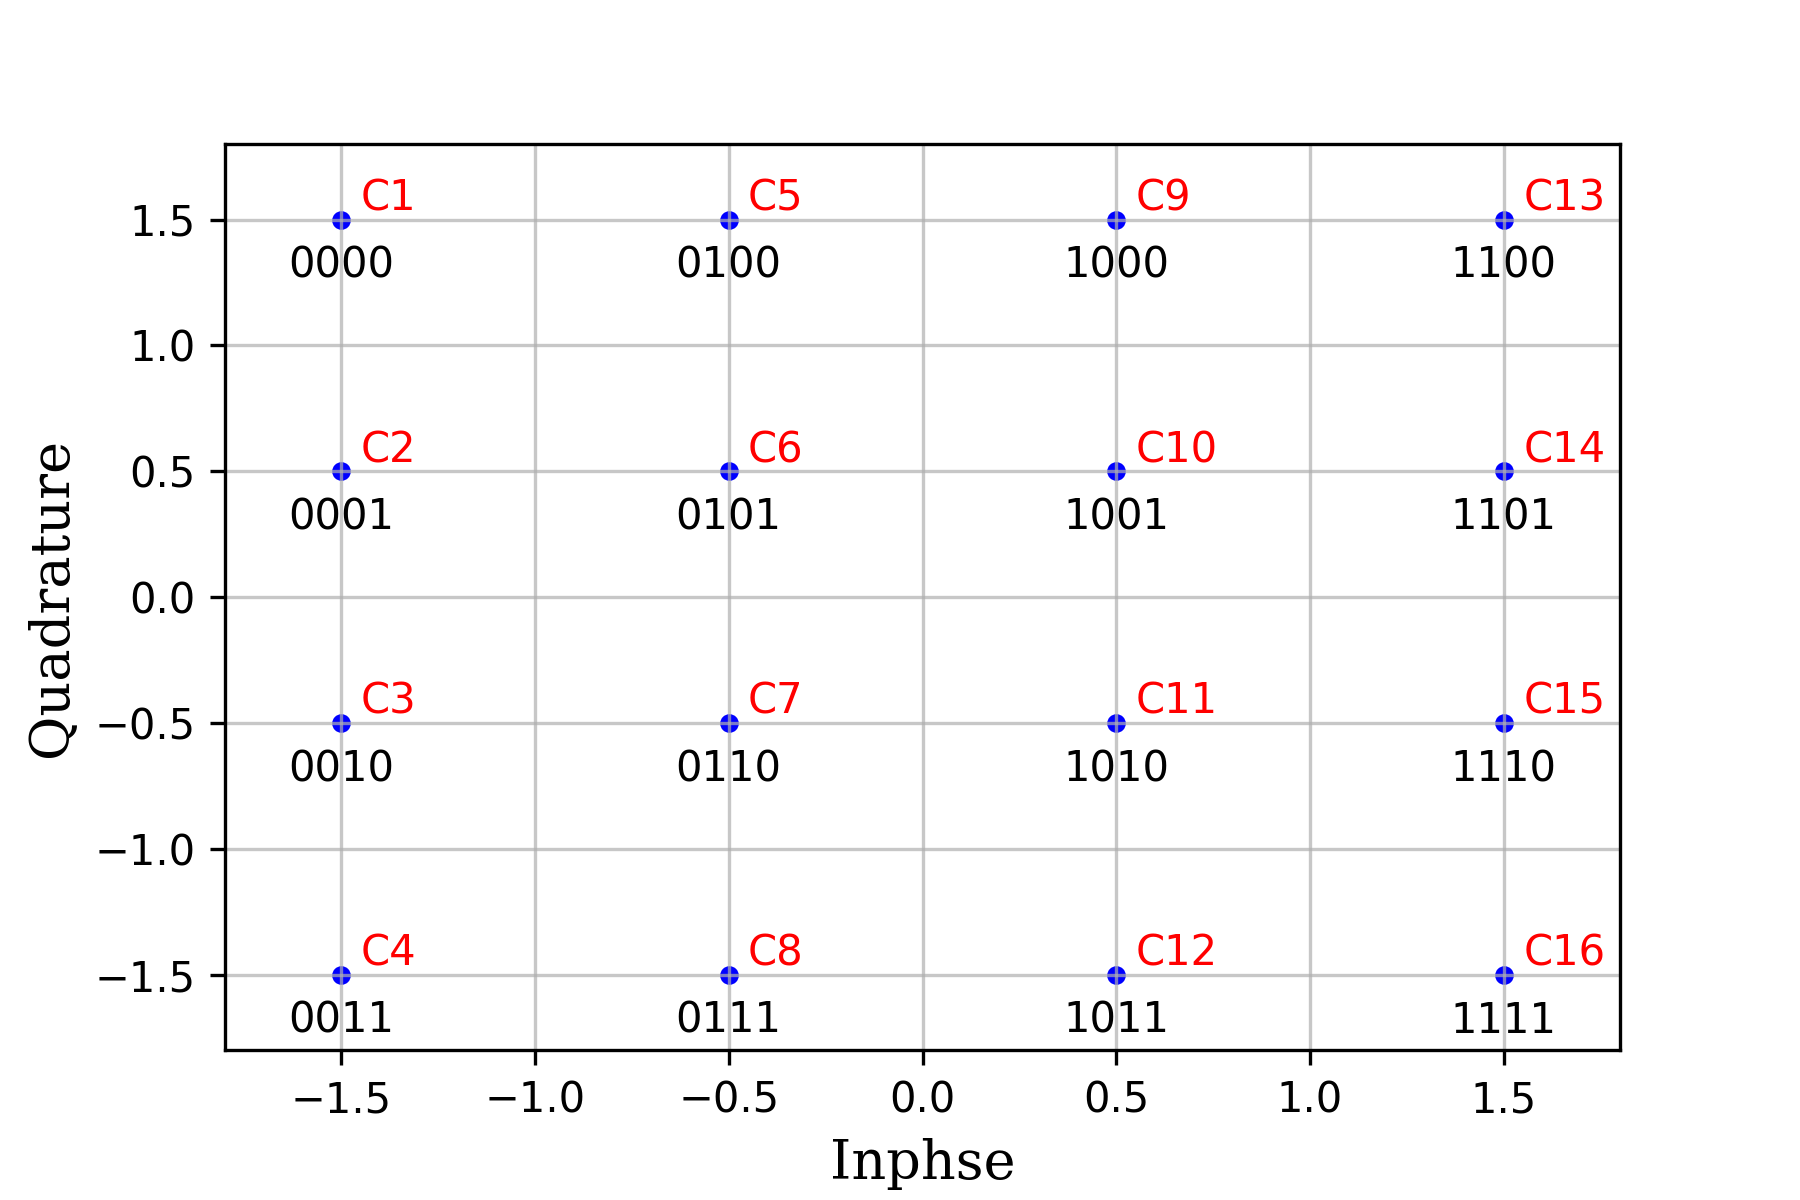
\includegraphics[width=0.6\linewidth]{QAMconsView}
\caption{Four bit per symbol signal represented in a phase diagram of a square 16QAM constellation. }
\label{fig:16QAMcons}
\end{figure}

\section{Electromagnetic Theory of Light}

The current theory of light comes from the idea of photons as the smallest unit of radiation composed of electromagnetic energy. As described by quantum mechanics a photon can be represented either by a wave or a particle. For the propagation and nonlinear interaction it is convenient to work in the wave picture, while at the detector you detect individual particles. A photon can be represented by  an electromagnetic field that arises from a set of coupled vector fields that are functions of time and position: the \emph{electric field} $\textbf{E}(\textbf{r},t)$  and the  \emph{Magnetic field} $\textbf{H}(\textbf{r},t)$. The phenomenological description of the interaction between this fields  are known as the \emph{Maxwell's equations} which describe all electromagnetic phenomena~\cite{FiberAgrawal}. 
\subsection{Maxwell Equations in a Medium}

In this thesis, the interaction between a modulated optical signal and silica glass fiber is studied to get a better understanding of nonlinear noise that corrupts an optical communication system. For a fundamental understanding, it is necessary to take into account the physical interaction of the medium with the electromagnetic field. A mediums response in the presence of a electromagnetic field is described by two vector fields: the \emph{electric flux density} $\textbf{D}(\textbf{r},t)$ and the \emph{magnetic flux density} $\textbf{B}(\textbf{r},t)$. For an optical communication system we can assume an optical fiber that is a nonconducting medium and has no free charges or currents, simplifying the interaction. These four fields are related by the  Maxwell's equations in a source-free medium~\cite{FundPhoto,FiberAgrawal}:

%lok at the notaciion

\begin{subequations}
\begin{gather}
\nabla \times \textbf{E }= -\frac{\partial \textbf{B}}{\partial t}\\
\nabla \times \textbf{H }= \frac{\partial \textbf{D}}{\partial t}\\
\nabla \cdot \textbf{D}= 0\\
\nabla \cdot \textbf{B}= 0
\label{eq:maxwell}
\end{gather}
\end{subequations}


The electric flux density $\textbf{D}$ relation to electric vector field $\textbf{E}$ is dependent on the properties of the medium, that are characterized by the \emph{polarization density} $\textbf{P}$. For a dielectric medium the polarization density is the sum of the electric dipole moments induced by the electric field~\cite{FundPhoto}. In an analog manner, the magnetic flux density $\textbf{B}$ relationship with the magnetic field $\textbf{H}$ is dependent on  the \emph{magnetization density} $\textbf{M}$ that describes the properties of the material. The connection between the vector fields and the flux densities  are given by

\begin{subequations}
\begin{gather}
\textbf{D}=\epsilon_0 \textbf{E}+\textbf{P}\\
\textbf{B}=\mu_0\textbf{H}+\textbf{M}%check
\end{gather}
\end{subequations}
where $\epsilon_0$ and $\mu_0$ are the vacuum permittivity and permeability respectably. Due to the nonmagnetic nature of silica glass, an optical fiber has $\textbf{M}=0$. When operating far from the mediums resonance, a phenomenological relation between  \textbf{P} and \textbf{E} can be used. This is the case for a optical fiber since we are interested in working in the low-loss wavelength region far from resonance.

In this project, nonlinear effects are the main objective, but it is necessary to have a description of linear dispersion effects as well. For a dispersive medium with a \emph{electric susceptibility }$\chi$  the relation between \textbf{P} an \textbf{E} is given as\cite{FiberAgrawal}:
\begin{equation}
\textbf{P}(\textbf{r},t)=\epsilon_0 \int^{\infty}_{-\infty} \chi(\textbf{r},t-t^\prime)\textbf{E}(\textbf{r},t^\prime)dt^\prime
\end{equation}
this response is dynamic, given that the electric field induces the bound electrons to start oscillating, and collectively create the polarization density. Given the oscillatory  response of the bound electrons, different harmonics can be reached. The electric susceptibility describes the strength of different harmonic components in respect to the incoming field.


In the simplest case of a \emph{linear}, \emph{nondispersive}, \emph{homogeneous} and \emph{isotropic} dielectric medium the the vectors \textbf{P} and \textbf{E} are parallel and proportional for every position and time, such that $\textbf{P}=\epsilon_0\chi\textbf{E}$~\cite{FundPhoto,FiberAgrawal}. Using the definition of the electric flux density \textbf{D} the \emph{electric permittivity} of the medium can be computed as $\epsilon=\epsilon_0(1+\chi)$, which for a nonmagnetic material is connected to the refractive index as $n=\sqrt{\epsilon/\epsilon_0}=\sqrt{1+\chi}$. From now on all materials discussed are \emph{homogeneous} and \emph{isotropic} making the relation between \textbf{P} and \textbf{E} independent of position \textbf{r} and independent from the direction of  \textbf{E}. Drawing some insight from the linear interaction response, a nonlinear dielectric media can be understood as an extension of this case. By considering a small change to the polarization density due to higher order oscillatory dependencies of the electric field and the medium. 


\subsection{ Nonlinear Dielectric Media}\label{sec:NLDM}

 Linear dielectric media gives a framework that can be extended to take into account higher order components of the electric susceptibility interaction with nonlinear orders of the electric field.  Let us consider the electric field vector $\textbf{E}(t)$, only time dependent, as a single harmonic electric field of angular frequency $\omega$ and complex amplitude $\mathcal{E}(\omega)$ written as~\cite{FundPhoto} 
 
\begin{equation}
\textbf{E}(t)= \textbf{Re}\left\{\mathcal{E}(\omega)e^{i\omega t}\right\}=\frac{1}{2}\left[\mathcal{E}(\omega)e^{i\omega t}+\mathcal{E}^*(\omega)e^{-i\omega t}\right].\label{eq:elfield}
\end{equation}
This electric field propagates through a medium as dictated by Maxwell's equations, thus the polarization density describes the mediums response. 

Inter atomic or crystalline field forces are much greater than the externally applied optical field, such that nonlinearity is usually weak. Thus, the relation between $\textbf{E}$ and $\textbf{P}$ is  approximately linear for small $\textbf{E}$, shifting slightly from linearity as $\textbf{E}$ increases. For a homogeneous isotropic dielectric medium the polarization density can be expanded as a power series around $\textbf{E}(t)=0$,  as done in Equation~\ref{eq:TayPden}~\cite{FundPhoto}.


\begin{tcolorbox}[title=Nonlinear Polarization Density Frequency Response]
\emph{The polarization density for a nonlinear dielectric medium is expressed as the sum of the linear component $(\epsilon_0\chi\textbf{E})$ and the nonlinear component $(\textbf{P}_{NL})$, which describes the medium's response to an incident electric field. }
\begin{subequations}
\begin{gather}
\textbf{P}(t)=\epsilon_0\left(\chi\textbf{E}(t)+2\chi^{(2)}\textbf{E}^2(t)+4\chi^{(3)}\textbf{E}^3(t)+\dotsm\right)\label{eq:TayPden}\\
\textbf{P}=\epsilon_0\left(\chi\textbf{E}(t)+\textbf{P}_{NL}(t)\right) , \ \ \ \textbf{P}_{NL}(t)=\left(2\chi^{(2)}\textbf{E}^2(t)+4\chi^{(3)}\textbf{E}^3(t)+\dotsm\right)
\end{gather}
\end{subequations}
\end{tcolorbox}
It is enough to take into account the first three terms  of the series, linear relation, second order and third order effects to describe the mediums response. The rest of the higher order effects have a very small contribution and can usually be ignored. 

It becomes necessary to distinguish between media that have second order or third order effects. A centrosymmetric medium presents dominant nonlinear optical processes described by the terms in the polarization density that are a cubic function of the electric field ~\cite{levenson1974dispersion}. In noncentrosymetric media, the polarization density exhibits dependencies on both the  squared and cube of the electric field. Throughout this project, our main concern is studying fiber optics made out of centrosymmetric media like fused silica SiO$_2$, such that nonlinear effects arise from third order nonlinear dependencies of the polarization density.

\subsection{Third Order Nonlinear Kerr effect}
Given this projects interest in centrosymmetric media it is necessary to describe the nonlinear response of the polarization density to an ideal monochromatic electric field like the one given in Equation~\ref{eq:elfield}.  Lets consider only the effects of the third order response of the dielectric medium $\textbf{P}_{NL}(t)=4\chi^{(3)}\textbf{E}^3(t)$. Substituting Equation~\ref{eq:elfield}  into the nonlinear polarization density  gives Equation~\ref{eq:PNL}, which describes the frequency response that arises.

\begin{tcolorbox}[title=Nonlinear Polarization Density]
\emph{The nonlinear polarization density $\textbf{P}_{NL}$ response to a monochromatic field can be decomposed into the individual frequency effects $\mathcal{P}_{NL}(\omega_i)$ that emerge from a third-order nonlinear medium~\cite{FundPhoto}.}
\begin{subequations}
\begin{gather}
\textbf{P}_{NL}(t)= \textbf{Re}\left\{\mathcal{P}_{NL}(\omega)e^{iwt}\right\}+\textbf{Re}\left\{\mathcal{P}_{NL}(3\omega)e^{i3wt}\right\}\\
\mathcal{P}_{NL}(\omega)=3\epsilon_0\chi^{(3)}|\mathcal{E}(\omega)|^2\mathcal{E}(\omega)\label{eq:wres}\\
\mathcal{P}_{NL}(3\omega)=\epsilon_0\chi^{(3)}\mathcal{E}^3(\omega)
\end{gather}
\label{eq:PNL}
\end{subequations}
\end{tcolorbox}

Two different frequency components $\omega$ and $3\omega$ emerge from the nonlinear response of the polarization density. The presences of a $3\omega$ response indicates that \emph{third-harmonic generated} (THG) light can be produced in the nonlinear interaction. However, in this cases the energy conversion efficiency is low for THG, 
producing a relatively weak $3\omega$ signal from the third order polarization density~\cite{FundPhoto}.
 
As has been mentioned before it is assumed that the polarization density response varies only slightly from the linear response $\epsilon_0\chi\textbf{E}$ with increasing \textbf{E}. It can be assumed that for a centrosymmetric material  an incremental change $\Delta\chi$ would be connected to the nonlinear polarization density \cite{FundPhoto,FiberAgrawal}. With this insight a similar assumption to the linear case can be made for $\mathcal{P}_{NL}$, relating it to the change in the susceptibility $\Delta\chi$ at a frequency $\omega$ by 
\begin{equation}
\mathcal{P}_{NL}(\omega)=\epsilon_0\Delta\chi\mathcal{E}(\omega).\label{eq:incPE}
\end{equation}

Expressing the incremental susceptibility as a change in the refractive index would be useful given the ease of measuring the refractive index in general. Since $n^2=1+\chi$, computing the deferential change would give $2n\Delta n = \Delta\chi$. It is also necessary to define the optical intensity of the electric field  given by $I=|\mathcal{E}(w)|^2/2\eta$ where $\eta$ is the impedance of the dielectric medium. With this and Equation~\ref{eq:incPE} the incremental refractive index can be written as a function of the optical intensity.
\begin{subequations}
\begin{gather}
\frac{\mathcal{P}_{NL}(\omega)}{\epsilon_0\mathcal{E}(\omega)}=2n\Delta n \rightarrow \Delta n= \frac{3\chi^{(3)}|\mathcal{E}(\omega)|^2}{\epsilon_0 2n}\\
\Delta n =\frac{3\eta}{\epsilon_0 n }\chi^{(3)}I\equiv \bar{n}_2 I
\end{gather}
\label{eq:Deltan}
\end{subequations}
\noindent Given the proportionality between the refractive index $\Delta n $ and the intensity $I$, the overall refractive index has a linear dependency of the optical intensity. This effect is known as the \emph{Optical Kerr Effect}~\cite{stolen1973optical}. 



\begin{tcolorbox}[title=Optical Kerr Effect]
\emph{ All material have a linear dependency on the optical intensity for high enough power, known as the Optical Kerr Effect. The effect arises from the anharmonic response of bound electrons to optical fields, resulting in a nonlinear susceptibility. The nonlinear coefficient $\bar{n}_2$ is also defined as the optical Kerr coefficient, but is also commonly known as the nonlinear-index coefficient.~\cite{FiberAgrawal,boyd2003nonlinear}  }
\begin{subequations}
\begin{align}
\bar{n}_2&=\frac{3\eta_0}{n^2\epsilon_0}\chi^{(3)} &  &\text{Optical Kerr Coefficient}\\
n(I)&=n+\bar{	n}_2I  &  &\text{Optical Kerr Effect}
\end{align}
\end{subequations}
\end{tcolorbox}

The optical Kerr effect makes a medium sensitive to power fluctuations. It is expected that some sort of distortion will be manifested in the signal due to its effect. In optical communication the Kerr effect induces nonlinear sources of noise that limit the system. To get a better understanding on the nonlinear effects it is necessary to study the properties of an optical fiber.




\section{Optical Fiber Overview}
In this section the phenomenological description for the optical fiber used to construct the communication links are discussed. To investigate nonlinear noise it is necessary to have a physical description of the interaction between the optical signal and the transporting fiber. First a few comments are made on the usual fiber refractive index profile and the definition of some fundamental properties, like the propagation constant of the medium. To describe the nonlinear interaction an extension will be made to the linear polarization density to include higher order terms. A general overview of the physics will be done, since a more detailed presentation is out of the interest of this thesis. 


\subsection{Fiber Properties}\label{sec:Fiber} 
\subsubsection{Refractive index fiber profile}

An optical fiber in a ray optics frame work is just a clever exploitation of the law of refraction and the critical angle.  In Figure~\ref{fig:FiberProf} a step index fiber profile is visualized, that has a refractive index $n_1$ in the core and $n_2$ in the cladding. The light gathering capacity of an optical fiber is known as the \emph{numerical aperture} (NA) that can be approximated for a step index fiber by 
\begin{equation}
\text{NA}=n_1(2\Delta)^\frac{1}{2}, \ \ \Delta=\frac{n_1-n_2}{n_1}
\end{equation}
where $\Delta$ is the \emph{fractional index}. Increasing the fractional index would improve the amount of light gather by the fiber, but it would also induce a large multipath or \emph{modal dispersion}. Figure~\ref{fig:FiberProf} shows a set of propagating rays, each traveling a path of different length. As a result, these rays disperse in time, broadening the pulse. Current optical communication fibers are design to have a $\Delta < 0.01$  allowing for better modal dispersion performance~\cite{FiberAgrawal}.  
\begin{figure}[H]
\center
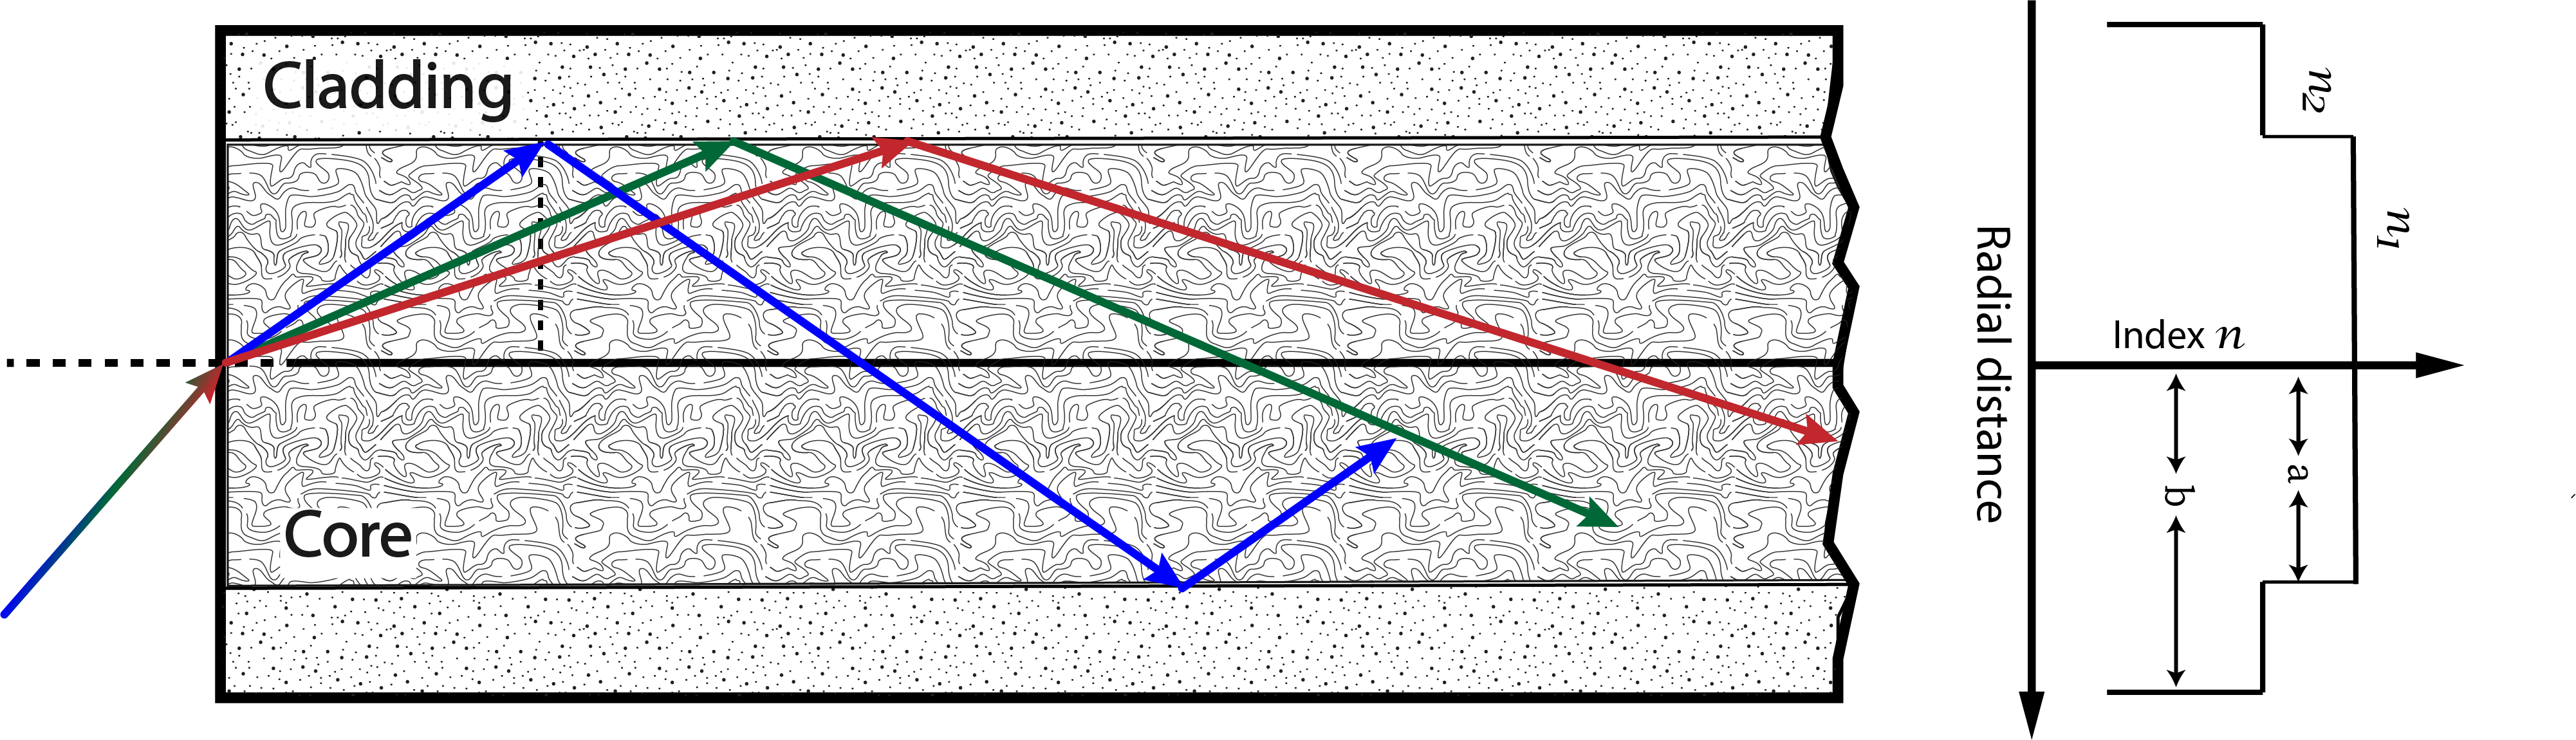
\includegraphics[width=\linewidth]{stepindexfibertotal}
\caption{A step index fiber with its corresponding refractive index profile is shown. Modal dispersion is visualized with a set of propagating rays that enter the fiber at the same time and would exit dispersed in time.  }
\label{fig:FiberProf}
\end{figure}
~
In Figure~\ref{fig:FiberProf} the \textit{refractive index profile} of the step index fiber is also shown. The core design plays an important role defining the fibers response to an optical signal. In Section~\ref{sec:ManOpF} the refractive index profiles of more interesting fibers will be discussed. 



\subsubsection{Power loss and Amplification}
A critical parameter for an optical system is the attenuation of the fiber. It provides a measurement of the power loss during transmission. For a communication system, having a strong output signal is important to reliably detect the transmitted signal. An optical fiber of length $L$ with an input launch power $P_0$ has a transmitted power $P_T$ written as 
\begin{equation}
P_T=P_0e^{-\alpha L},
\end{equation}
where $\alpha$ the \emph{attenuation constant} is a measure of all the losses in the fiber~\cite{agrawal2000nonlinear}. The attenuation constant has units of dB/km and is wavelength dependent, as reported in Reference~\cite{miya1979ultimate} a fiber with $\Delta=1.9\cdot10^{-3}$ exhibits a fiber-loss of 0.2~dB/km in the wavelength region near 1550~nm. In today's optical communication system the usual operating frequency $\omega$ is 193.1~THz because of its low fiber-loss and ease of amplification using \textit{erbium doped fibers}.

Amplification is crucial to counteract the losses in the fiber, extending the reach of the communication system. An ideal amplifier would produce an output power $P_{out} = G P_{in}$ without distortion given an input power $P_{in}$. In general an amplifier can be described by the  \textit{amplification factor} $G(\omega)$ and the \textit{amplification profile} $g(\omega)$ given by $G=e^{gL}$. The amplifiers simulated imparted a minimum amount of noise, having a low \textit{noise figure} of 3~dB. Thus, the dominant sources of noise will arise from the light-matter interaction.



\subsubsection{Chromatic dispersion}\label{sec:CD}

When electromagnetic waves interacts with a medium's bound electrons, different effects arise through the polarization density, some of which have been covered is Section~ \ref{sec:NLDM}. The interaction between the atomic structure and the electromagnetic field is also dependent on the fields frequency $\omega$. This property is known as \textit{chromatic dispersion}. The frequency dependence is manifested through the refractive index $n(\omega)$. Far from the material resonance the refractive index can be approximated by the \emph{Sellmeier equation}~\cite{agrawal2000nonlinear,FiberAgrawal}

\begin{equation}
n^2(\omega)=1+\sum^m_{j=1}\frac{B_j\omega^2_j}{\omega^2_j-\omega^2}
\end{equation}
 where $\omega_j$ is the resonance frequency and $B_j$ is the strength of the jth resonance. In a optical fiber these parameters are found experimentally by fitting the material dispersion curve. Fiber dispersion plays a critical role when building an optical communication system. A pulsed signal frequency components can be found through the Fourier transformation of the signal in the time domain, as is known form signaling theory a pulsed signal contains a range of frequencies. In the same manner, transmitted light pulses are composed of frequencies, in a dispersive medium each frequency would travel at its unique speed $c/n(\omega)$ making the pulse spread in time.
 
 When nonlinear effects are present in the fiber as well, the combination of dispersion and nonlinearity can result in a more complex behavior. This will be discussed in Section~\ref{sec:NLPN}. The fiber dispersive effects are dependent on the mediums \textit{propagation constant} $\beta$ defined as 
 

\begin{equation}
\beta(\omega)=n(\omega)\frac{\omega}{c}.
\end{equation}
An approximate response for the complete spectral range can be obtained by doing a Taylor expansion around the pulse center frequency $\omega_0$
\begin{equation}
\beta(\omega)=\beta_0+\beta_1(\omega-\omega_0)+\frac{1}{2}\beta_2(\omega-\omega_0)^2+\dotsm
\end{equation}
where the frequency derivatives of the propagation constant are given by 

 \begin{equation}
\beta_m=\left(\frac{d^m\beta}{d\omega^m}\right)_{\omega=\omega_0} \ \  m=0,1,2...,
\end{equation}
and are related to different fundamental properties of the fiber. Due to the pulses spectral composition it propagates with a \emph{group velocity}  defined as $\nu_g=(d\beta/d\omega)^{-1}$ ~\cite{born2013principles}. It can be expressed in function of the refractive index  as
\begin{equation}
\frac{1}{\nu_g}=\beta_1=\frac{d}{d\omega}n(\omega)\frac{\omega}{c}=\frac{1}{c}\left(n+\omega\frac{dn}{d\omega}\right)=\frac{n_g}{c}\label{eq:beta1}
\end{equation}
where the \emph{group refractive index} is $n_g=\left(n+\omega\frac{dn}{d\omega}\right)$. Given the mediums frequency dependence different frequency components undergo different delays. This effect is known as \textit{group velocity dispersion} (GVD)~\cite{agrawal2000nonlinear}, the fibers dispersive effect  is described by the \emph{dispersion parameter} $D$ either in terms of wave length $D_\lambda$  or frequency  $D_\omega$ differing by a factor of $d\omega/d\lambda=-2\pi c /\lambda^2$. 
\begin{equation}
D_\lambda=\frac{d\beta_1}{d\lambda}=-\frac{2\pi c}{\lambda^2}\beta_2
\end{equation}

The units for $D_\lambda$ are [s/m-Hz] and for $D_\omega$ has [ps/nm-km] presenting variation in value given a wavelength. Thus, a pulse spectrum would under go slightly different values of $D$ which would broaden the pulse. This broadening is a higher-order dispersive effects governed by the \emph{dispersion slope}   $S=dD/d\lambda$ that can be written in terms of propagation constant $\beta_2$ and $\beta_3$ as
\begin{equation}
S=\frac{2\pi c}{\lambda^2}\beta_3+\frac{4\pi c}{\lambda^3}\beta_2.
\end{equation}

An optical fibers cladding/core can be designed in such a way that the total dispersion of the fiber can present desirable properties for an communication system. With a clever design, the fibers dispersive response can be flattened to a have a constant value for a spectral range. Another fiber can also be designed to have shifted a dispersion minimum present at frequency with lowest attenuation. 

Dispersion in an optical communication link can alter the signals timing, due to the pulse broadening in time different pulses would start to overlap, distorting the signal. Optical compensation can be done using fibers with opposite dispersion parameters  to cancel each others effect out. It is more useful to use a highly dispersive fiber to compensate in a short length a large amount of accumulated dispersion. A more detailed description of dispersion compensation is done in Section~\ref{sec:DisCom}.  

\subsection{Higher Order Optical Noise}\label{sec:NLPN}
A silica fiber presents a linearly dependent refractive index due to the optical Kerr effect. As is discussed by S. Dris et al. in Reference~\cite{dris2017analysis} ''\textit{Nonlinear interference noise} (NLIN) due to the Kerr effect presents the most significant bottleneck towards increasing throughput in a flexible WDM optical networks''. The objective of this project is to suggest a detection scheme that mitigates NLIN.  Through this section a description of the different noise sources of interest will be presented. 

First, it is necessary to define quantities that represent the signals resilience.  The signals quality is quantified by  \textit{optical signal to noise ratio} (OSNR) that is dependent on the signal power $P$ and noise average power $N$ given by
\begin{equation}
\text{OSNR}=10\log_{10}\left(\frac{P}{N}\right)
\end{equation}
 in dB units~\cite{FiberAgrawal}. In a coherent system it is necessary to have a high OSNR at the receiver, usually above 20~dB, for an accurate detection. When noise is present, either linear or nonlinear, the OSNR drops, distorting the signal. As discussed in the introduction, the NLIN distortion is present as a phase noise rotation preserving some information. 
 
 In a communication system the quality of the transmission relies on the amount of correctly classified symbols. With a low number of misclassified symbols, correction can be implemented in a higher layer of the communication system to recover or correct bit stream transmitted with FEC~\cite{NLPNinCFO}. The SER describes the amount of mistakes made in the total transmitted signal as
 \begin{equation}
\text{SER} = \frac{\text{no. of incorrect received symbols}}{\text{no. of transmitted symbols}}.
\end{equation}

Nonlinear noise in an optical communication system induces a phase shift to the detected signal. If not taken into account, it becomes a fundamental limiting factor to the transmission distance~\cite{NLPNDSP}. Having a physical description of the different nonlinear effects, is then useful to alter the expected detection regions to improve the SER.



 Three different nonlinear effects will be discussed that fall into  two categories, \emph{intra-channel NLIN} or \emph{self-channel interference} and \emph{inter-channel NLIN} or \emph{cross/multi-channel interference}. The intra-channel effects in interest are \emph{self phase modulation } and the \emph{Gordon-Mullenauere effect}. For inter-channel effects \emph{cross phase modulation} will be considered in a WDM system.
  
\subsubsection{Self Phase Modulation}
In a fiber absent of dispersion $\beta_2=0$ the transmitted pulse undergoes a phase shift due to the intensity dependent refractive index, this modulation is known as \textit{self phase modulation }(SPM). The refractive index intensity dependence induces a power dependence on the propagation constant~\cite{FiberAgrawal}, that can be written as~\cite{le2015advanced}  

\begin{equation}
\beta^\prime=\beta+k\bar{n}_2\frac{P}{A_{eff}}=\beta+\gamma P ,\ \ \ \gamma = \frac{2\pi \bar{n}_2}{\lambda A_{eff}}
\label{eq:gammadef}
\end{equation}



where $A_{eff}$ is the effective area of the guided mode and $k=2\pi/\lambda$ is the wavenumber. In it self the change to the propagation constant suggest an effect analogues to GVD, where the pulse is chirped and spectral broadening~\cite{agrawal2000nonlinear}. As is deduced in Reference~\cite{le2015advanced} the total nonlinear phase shift can be computed as the difference between $\beta^\prime$ and $\beta$ over the interaction length as  
\begin{subequations}
\begin{gather}
\phi_{\text{SPM}}=\int_0^L(\beta^\prime-\beta)dz=\int_0^L\gamma P(z)dz\\
\phi_{\text{SPM}}<\gamma L_{eff}P_{in}.
\end{gather}
\label{eq:phinl}
\end{subequations}
The effective interaction length is defined as $L_{eff}=(1-e^{-\alpha L})/\alpha$ and the power in the fiber $P(z)=P_{in}e^{\alpha L}$~\cite{le2015advanced}. Equation~\ref{eq:phinl} gives us the amount of phase change over the fiber length L along the propagation axis $z$. The assumptions made to compute the nonlinear phase shift describes the maximum phase shift possible in a system where a CW driving laser is used with a IM/DD format non-return to zero (NRZ) ~\cite{agrawal2001applications,FiberAgrawal,le2015advanced}. 

It is important to note that when dispersion effects are present the dependencies become more complex and require more sophisticated numerical solutions, making it cumbersome to have a complete model of the system~\cite{agrawal2001applications,gordon1990phase}.  In multiple references ~\cite{le2015advanced,FiberAgrawal,agrawal2000nonlinear} the limit for $P_{in}$ is introduced as a general rule to follow before SPM starts to corrupt the signal.  The upper bound  is given as $P_{in}<0.1\alpha/\gamma N_{A}$, where $N_{A}$ is the number of amplifiers~\cite{le2015advanced}. For  an average fiber system with 10 amplifiers the upper limit is 1.2-3~mW. Making it a critical impermanent for optical system with a high average power. SPM is a NLIN and as concluded in Reference~\cite{dris2017analysis} the effects are modulation format independent.



\subsubsection{Cross Phase Modulation}
In a WDM system the presence of multiple channels in a single fiber span would alter the interaction of the fiber with the transmitted optical signal.  If we have an $M$-channel WDM system with a fixed channel spacing the cross-phase modulation for channel $i$ can be described as
 
\begin{equation}
\phi^i_{\text{XPM}}=\gamma L_{eff}\left(P^i_{in}+2\sum^M_{j\ne i}P_j\right)
\end{equation}
where we can see that SPM effects are also taken into account for each channel. The XPM  effects are important due to the dependence of the channels phase with the bit patterns of all the others~\cite{agrawal2001applications}. As in the case of SPM a phase shift can be computed to represents the maximum  shift acquired in a system 
\begin{equation}
\phi^i_{\text{XPM}}<\frac{\gamma}{\alpha}(2M-1)P_{ch}
\end{equation}
where $P_{ch}$ is the power per channel. Given the linear relation between the phase shift and the number of channels, there is a limitation to the number of channels or power per channel that can be transmitted.

 In a system where GVD effects are present, pattern-dependent phase shifts are converted to power fluctuations, reducing the OSNR at the receiver~\cite{agrawal2001applications}.  A rough estimate for the power restriction is computed in Referene ~\cite{le2015advanced} for maximum phase shift $\phi_{XPM}<1$~rad the upper bound is  $P_{ch}~<~\alpha/\gamma N_{A}(2M~-~1)$ before XPM effects arise. In general the power restriction per channel is limited to bellow 1~mW depending on the system, increasing the amount of constraints for the system design. Through this section no mention of the effect of amplification has been mentioned, the interaction between the spontaneous noise produced by amplification and the Kerr effect plays an important role in long-haul transmission links. 


\subsubsection{Gordon-Mollenauer Effect}

In a fiber communication link it is usual to use multiple segments of fiber with optical amplifiers (OA) to extend the systems reach. This type of architecture is known as lump amplification, commonly used in long-haul optical systems with over 10 amplifiers. Noise produced by OA interacts with the fiber through the Kerr effect  producing phase fluctuations at the receiver and limiting the transmission distance~\cite{agrawal2001applications}. This nonlinear source of noise is known as the \textit{Gordon-Mollenauer effect}~\cite{gordon1990phase} or simply \textit{nonlinear phase noise} (NLPN). 

A transmission line that has $N$ spans of optical fiber followed by its corresponding  linear loss amplification is ultimately limited by the presence of \textit{amplified spontaneous emission} (ASE) noise. Due to the refractive index dependence on optical power, fluctuation produced by ASE noise induces a phase shift in the received signal~\cite{gordon1990phase}. The nonlinear  fluctuation  can be approximated as ~\cite{le2015advanced}    

\begin{equation}
\phi_{\text{NLPN}}\approx N\gamma L_{eff}P_{in}.
\end{equation}

Notice that the ASE noise is still a linear source of noise added to the signal as AWGN. However, it also has a second effect by introducing small fluctuations in the optical power, inducing a phase shift in the transmitted signal due to the Kerr effect. As is explained by P. Gordon and L. Mollenauer in Reference~\cite{gordon1990phase} noise produced by the amplifier can be decomposed into a noise field with two degrees of freedom that have the same shape as the pulse. ''One in-phase with it, and the other in quadrature. The quadrature component produces an immediate phase shift, and the in-phase one alters the energy of the pulse. The energy change results in an additional nonlinear phase shift by the time the pulse reaches the receiver''.
\subsubsection{Compound Nonlinear Phase Shift}

Three sources of nonlinear interference noise have  been presented; self phase modulation, cross phase modulation and nonlinear phase noise. Each of this effects induces a phase shift to the transmitted signal. Represented in a phase diagram as a rotation of the transmitted constellation. Corrupting the detected phase. Each of the NLIN sources has a complex interaction with the dispersive effect, making it necessary to carry out a numerical simulation for a precise model. However, it is not always possible to know the systems parameters before hand, given that in a real system deploying a fiber link requires tolerances.

A maximum phase shift can be expressed for each of the noise source, adding  up to a total maximum nonlinear phase shift $\phi_{\text{nl}}$. A general approximation to quantify the expected phase shift for a signal can be computed as

\begin{equation}
\phi_{\text{nl}}=\phi_{\text{SPM}}+\phi_{\text{XPM}}+\phi_{\text{NLPN}}.
\end{equation} 
Each effect contributes to the total phase shift induced on the signal. Even though they all arise from the Kerr effect, some can be compensated more efficiently than others. Compensation in the end is what interest us, extracting as much transmission distance or capacity from the system before nonlinear noise corrupts the signal.  



        
\begin{tcolorbox}[title= Bound Nonlinear Phase Shift ]
\emph{All sources of nonlinear noise; XPM, SPM and NLPN are found to have an upper bound for a fixed system configuration. Thus, an upper bound can be set on the total nonlinear phase noise that is detected at the receiver side.  }
\begin{equation}
\phi_{nl}<\frac{\gamma}{\alpha}\left (2M+N\right )P_{ch}
\end{equation}
Where $\gamma$ is the nonlinear parameter defined in Equation~\ref{eq:gammadef} and $\alpha$ is the absorption coefficient of the fiber. A reference value can be drawn for a M-channel and N-span link, quantifying the nonlinear phase shift undergone by the signal.  
\end{tcolorbox}

\subsection{Optical Fiber and Compensation }
As presented in the previous section, nonlinear effects are quantified by some fundamental parameters; the  nonlinear refractive index, dispersion parameter and the dispersion slope. In Section~\ref{sec:Fiber} there properties were presented. However, it is also necessary to discuss the different types of fiber that can be manufactured and how they can be used to compensate for fiber dispersion.  In this section, the physical description for  dispersion compensation is introduced. We conclude by discussing the different fibers used for the simulation and how they where implemented.    
\subsubsection{Dispersion Compensation in Fibers}\label{sec:DisCom}
 All optical fibers manifest dispersive effects, given the  refractive index dependence on frequency. In Section~\ref{sec:CD} the dispersion coefficient was introduced, concluding that given the different frequency components of a optical pulse, would spread in time due to GVD altering the system's timing~\cite{goldfarb2007chromatic}. Compensation becomes then necessary to retrieve the original signal. Fortunately, a clever design of the optical core can alter the dispersion parameter $D_\omega$ and the dispersion slope $S$ such that a zero dispersion system can be constructed. Consider a link composed of two fibers, a \textit{single mode fiber }(SMF) with a $D_{1}$ and a \textit{dispersion compensating fiber} (DCF) with a $D_{2}$. The condition for perfect dispersion compensation is 
\begin{equation}
D_{1}(\lambda_{n})L_{1}+D_{2}(\lambda_{n})L_{2}=0\label{eq:DC}
\end{equation}
where $\lambda_{n}$ is the operating wavelength of the nth channel and $L_{i}$ is the corresponding length of each fiber. It is clear then that the dispersion compensation varies slightly for each channel. Thus, to have  perfect compensation it is necessary to also consider the slope of the dispersion coefficient. It would be ideal if the dispersion slope for the DCF could be design to have a value of
\begin{equation}
S_{2}=S_{1}\frac{D_{2}}{D_{1}}.\label{eq:SC}
\end{equation}
\indent Unfortunately, manufacturing and fiber design have limits, such that it is not usual to have a perfectly compensated link. When designing a communication system the dispersion scheme is built around the operating wavelength $\lambda=1550~nm$ (as has been mentioned before) this wavelength has a low absorption, presents zero dispersion in some fibers and is the current standard in optical communication. Thus, to design a link the fiber is first selected depending on the system's configuration. In practice it is desirable to have a DCF that has a dispersion coefficient and slope that best approximate the values given by Equations~\ref{eq:DC} and Equation~\ref{eq:SC}. 
\begin{figure}[h]
\center
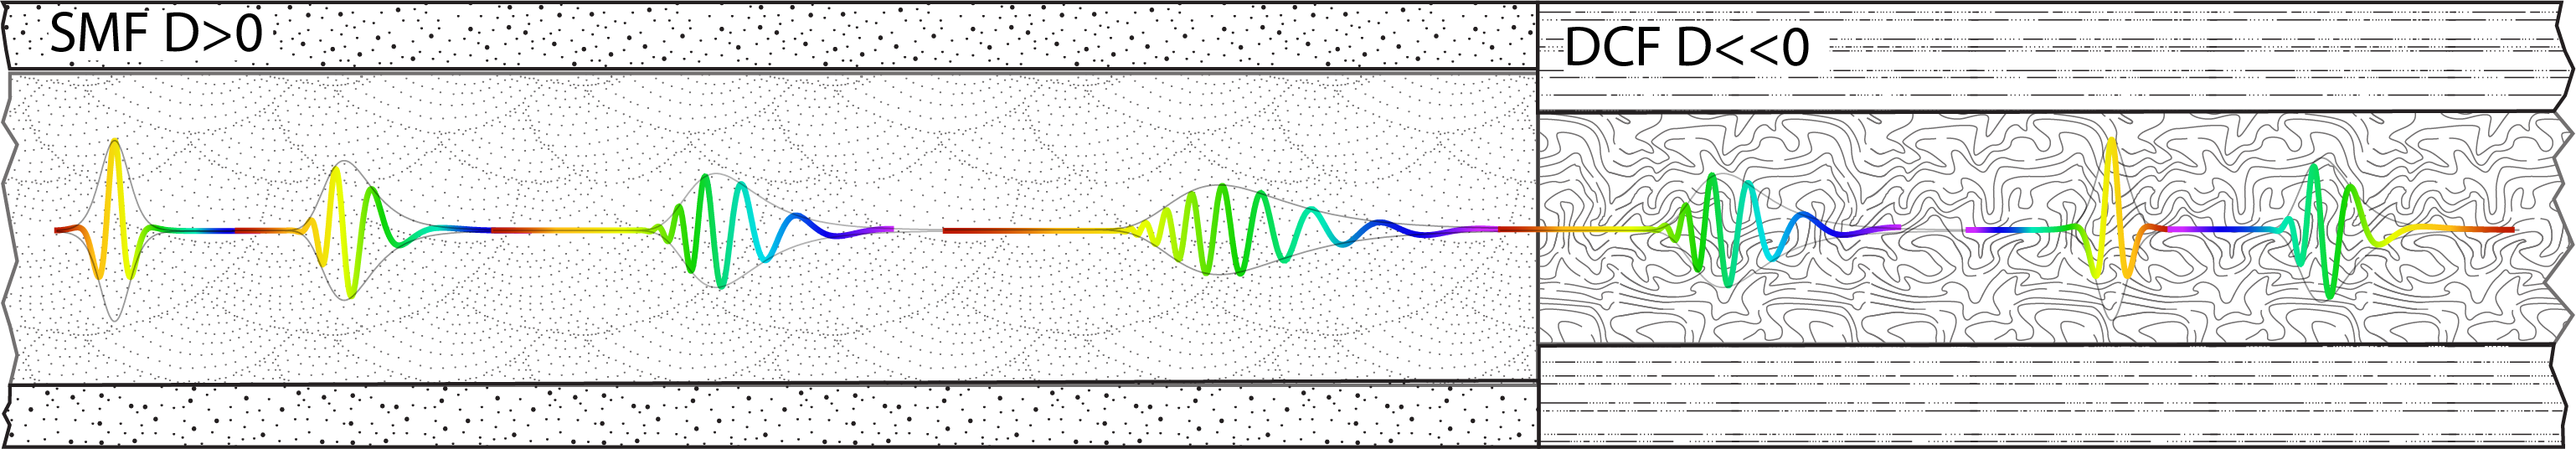
\includegraphics[width=\linewidth]{fiberdcf.png}
\caption{Visualization of chromatic dispersion of a optical pulse propagating through a SMF. Compensation of pulse was preformed using a highly dispersive DCF.  }
\label{fig:GVD}
\end{figure} 
A more accurate visualization of GVD is represented in Figure~\ref{fig:GVD} where a propagating pulse is spreading in time, compensation is also shown using a short DCF that mitigates the dispersion accumulated in a long SMF. Ignoring losses between fiber splices notice that the effective core area for a DCF is smaller than SMF. Making compensating fibers have a larger nonlinear refractive index $\bar{n}_{2}$, thus making NLIN more present in the system. 




\subsubsection{Manufactured Optical Fibers}\label{sec:ManOpF}

The refractive index profile can be designed to alter the optical properties of the fiber. In previous sections the connection between the refractive index and the dispersion coefficient, nonlinear coefficient and other parameters has been discussed. Now we are interested in making a few remarks about the optical fibers that were implemented during the simulation. Each fiber that was used in the simulation followed specifications from a real fibers that have been studied in peer-reviewed articles.
\begin{figure}[h]
  \centering
  \subfloat[DSF]{\label{fig:DSF}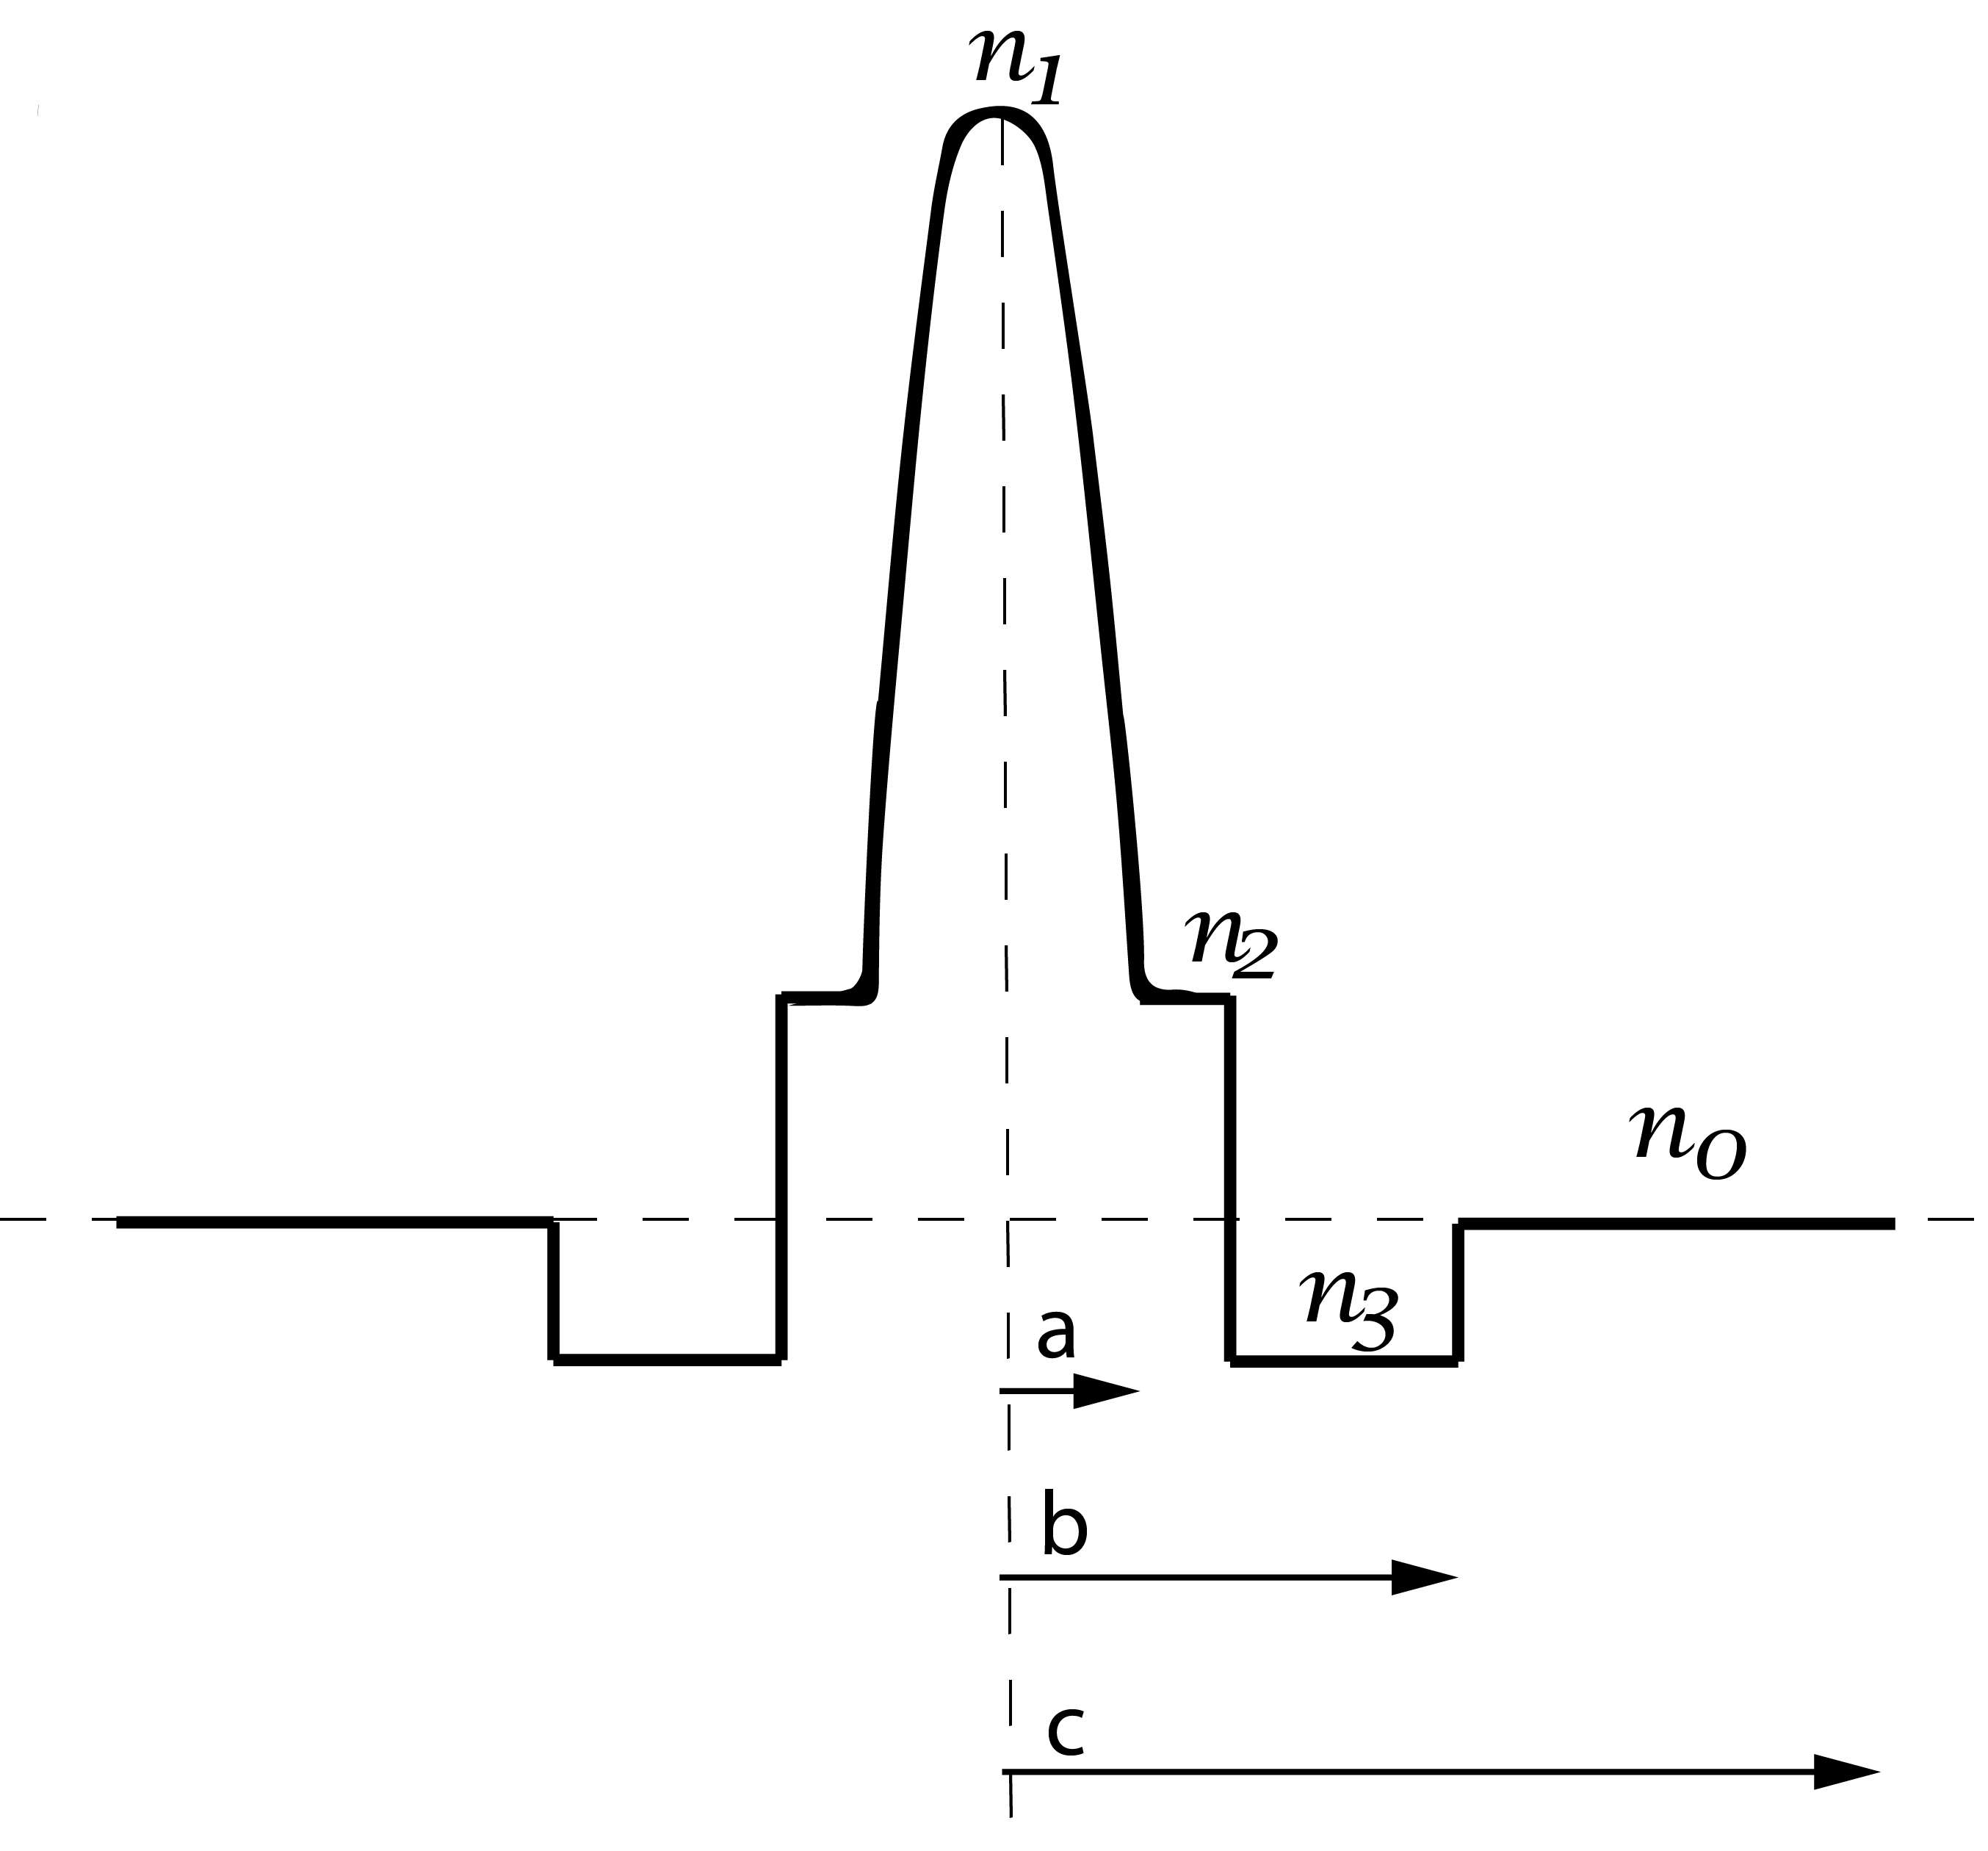
\includegraphics[width=0.45\textwidth,height=15em]{DSFprofile.png}}
  \qquad
  \subfloat[DCF]{\label{fig:DCF}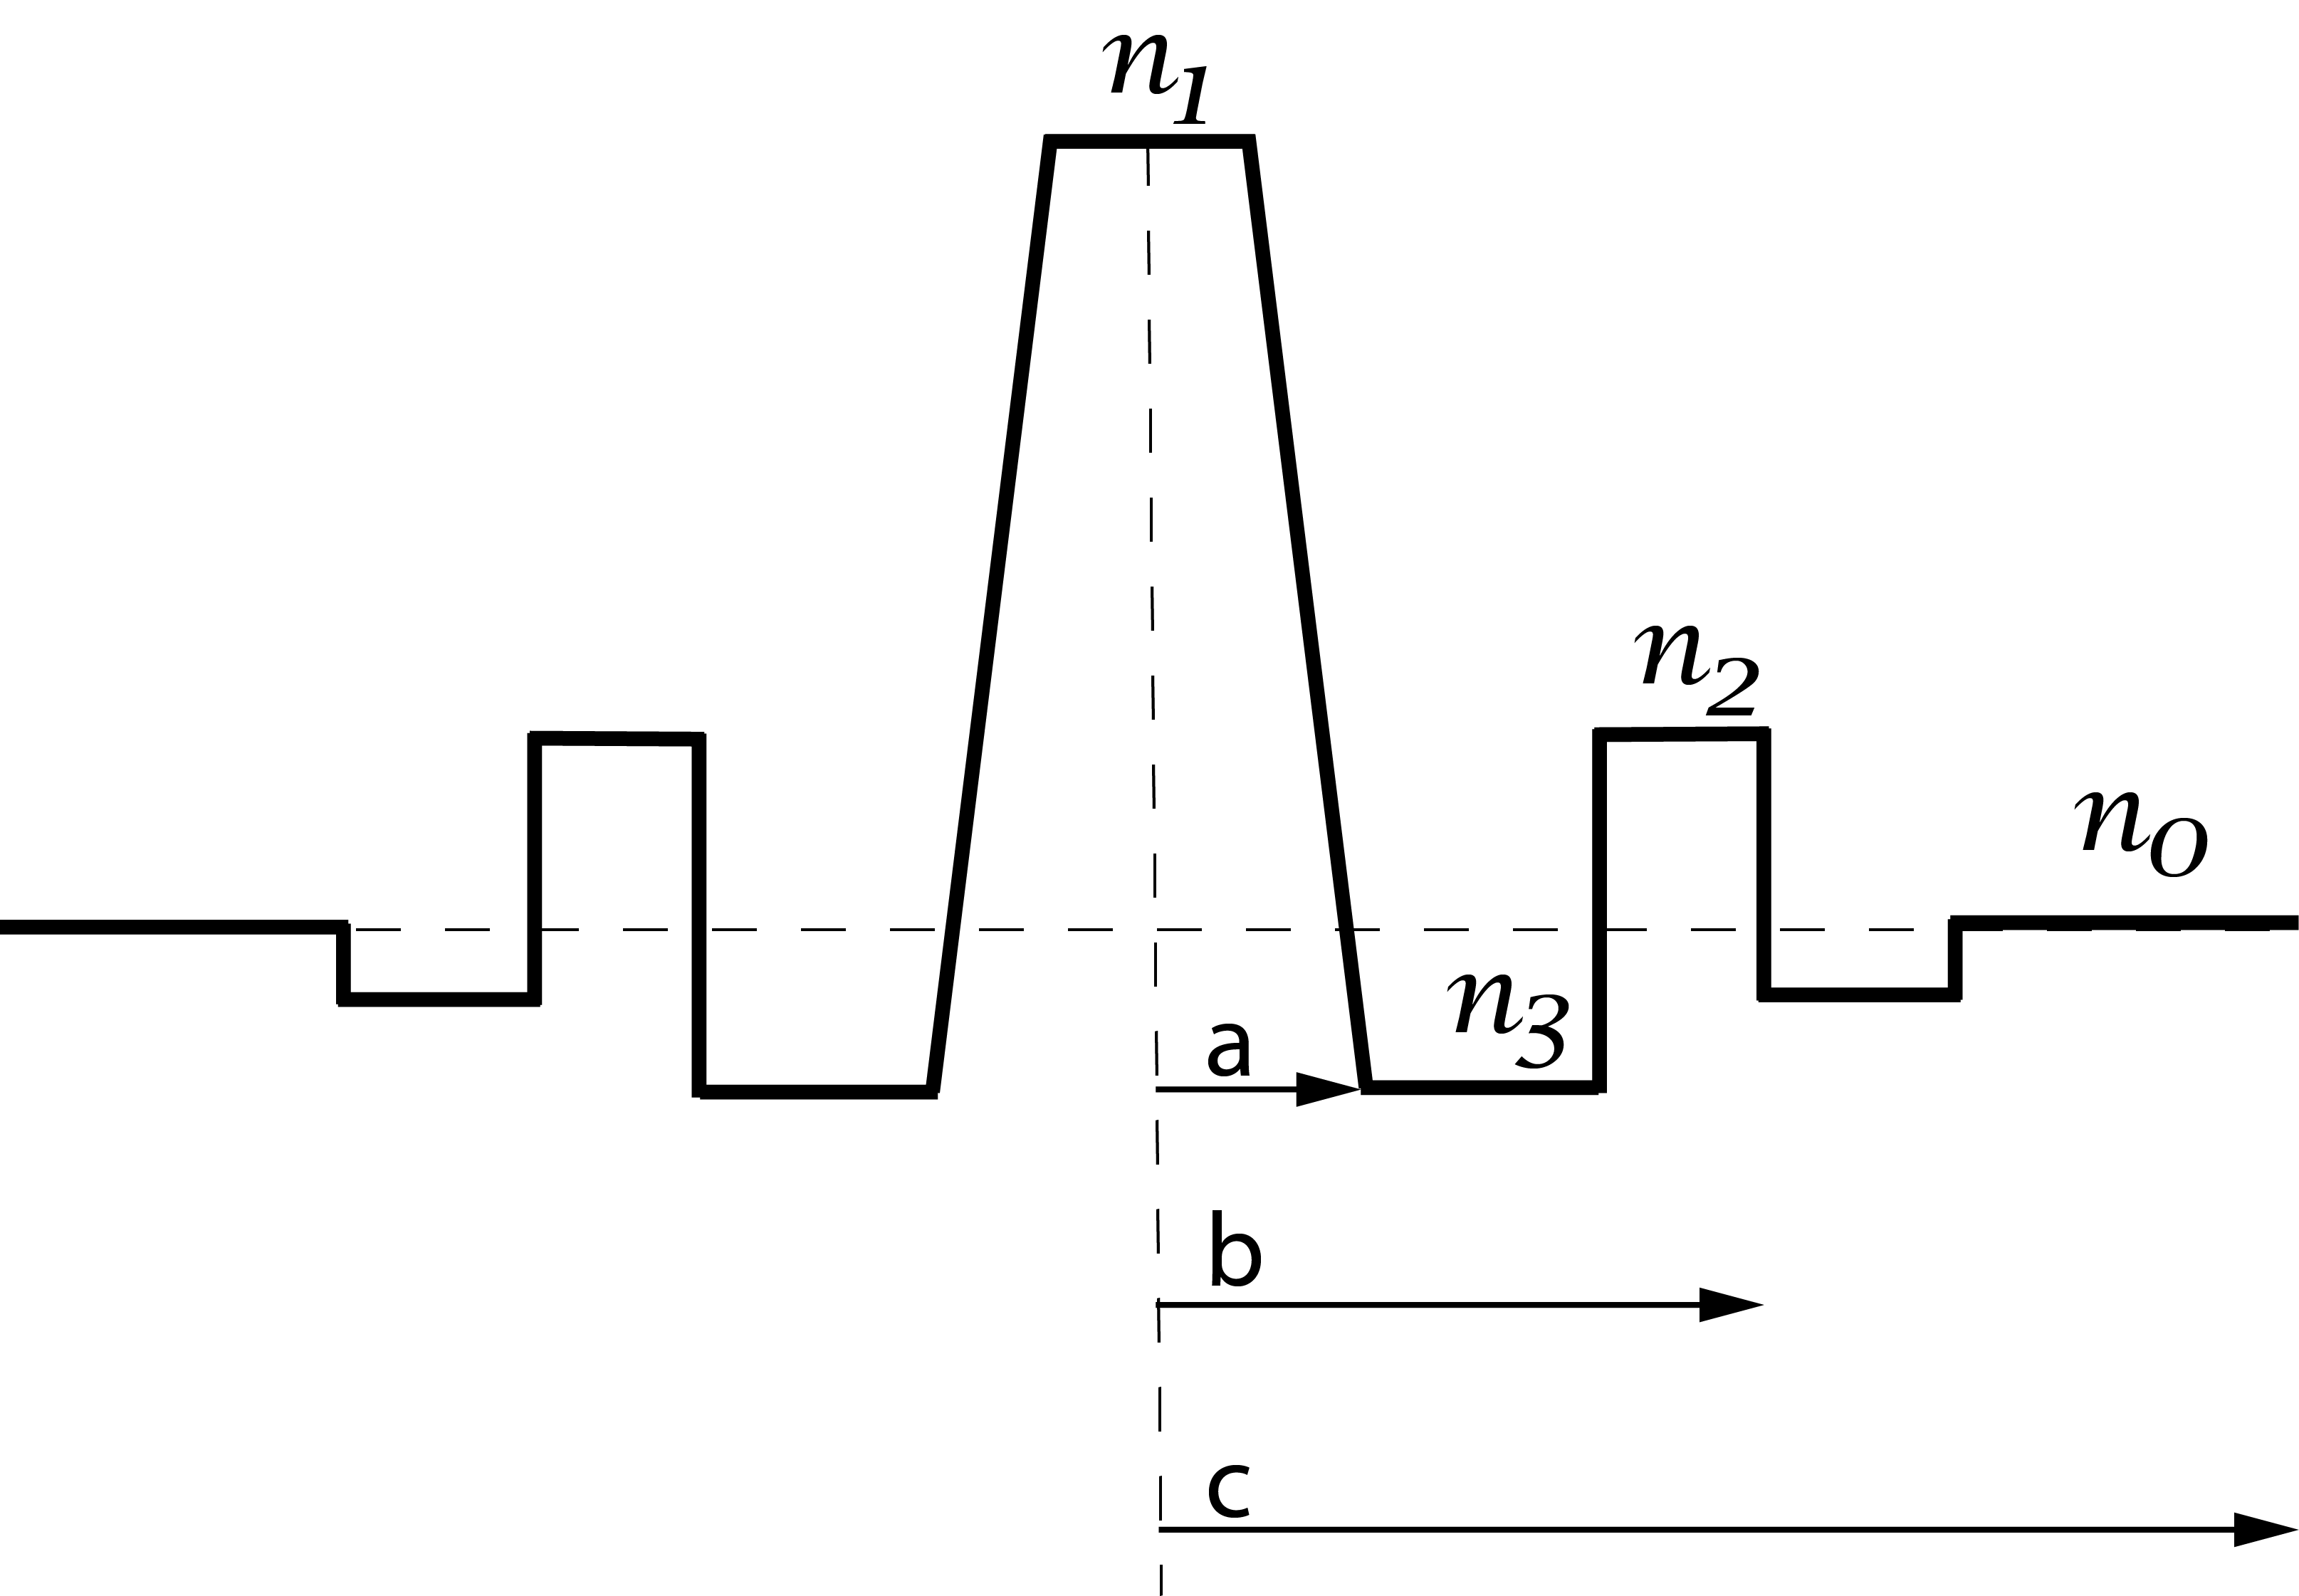
\includegraphics[width=.45\textwidth,height=15em]{DCFprofile.png}}     
  \caption{Refractive index profile for dispersion shifted or dispersion compensating fibers. \\ {\scriptsize Image designed inspired by available figures in Reference~\cite{kato2000dispersion,aikawa2005dispersion}}}
  \label{fig:FiberIndex}
\end{figure}

First, let us consider a single channel system with a operating wavelength of $1550~nm$. If only one channel is present then it would be useful that the fiber would have zero dispersion for this wavelength. Multiple fibers exist in the market that present zero dispersion for this wavelength, they are known as  \textit{dispersion shifted fiber} (DCF)~\cite{kato2000dispersion,kim1994measurement}. To design a optical fiber with a shifted dispersion the refractive index profile has to made in such away that the fibers chromatic dispersion and the waveguide dispersion balance each other out. The general refractive index profile is shown in Figure~\ref{fig:DSF}, compared to a step index fiber (Figure~\ref{fig:FiberProf}) four different cladding sections with different refractive index are used, this intricate design achieves modified dispersion effects. However, not all system architectures can use DSF given that when multiple channels are present in the same fiber it is necessary to compensate the dispersion acquired by all channels.


For WDM systems it is usual that all channels present dispersion in the transmission fiber. Instead of implementing a DSF a \textit{nonzero-dispersion shifted fiber} (NZ-DSF) is deployed that presents a small dispersion value for the center wavelength $1550~nm$. As was mention in Section~\ref{sec:DisCom}, it is not enough to just consider the dispersion parameter, it is necessary to take into account the dispersion slope as well to compensate a multichannel system. To compensate a separate \textit{slope compensating-dispersion compensation fiber} (SC-DCF) or SC-DCF module~\cite{aikawa2005dispersion} is used to compensate the acquired dispersion for all channels in a short span of fiber. Figure~\ref{fig:DCF} shows the refractive index profile for a general DCF, the fiber design is not trivial, but thanks to this clever design, dispersion is not a limiting factor for transmission distance as it once was.


\begin{mytable}[float=h, label=tab:FiberData]{ Fiber Characteristics}
\emph{Physical characteristics for the optical fibers used in the simulations. In the long-haul system the DSF is implemented and a combination of NZ-DSF and SC-DCF is used in the WDM system. }
\begin{center}
\begin{tabular}{c|cccccc} 
\toprule
Fiber& $\bar{n}_{2}$~$[10^{-20}\frac{cm^2}{W}]$ & $\alpha~[\frac{dB}{km}]$ & $A_{\text{eff}}~[\mu m^2] $  & $D~[\frac{ps}{nm-km}]$ & $S~[\frac{ps}{nm^2-km}]$   \\ 
\midrule
DSF & 2.4 & 0.21 & 70 & $<$0.13 & 0.11  \\ 
\midrule
NZ-DSF & 2.25 & 0.2 & 65 & 4.2 & 0.085  \\ 
\midrule
SC-DCF & 2.8 & 0.41 & 16.7 & -47 & -0.93  \\ 
\bottomrule
\end{tabular} 
\end{center}
All values used for the fiber design in the simulation where taken from References~\cite{kato2000dispersion,kim1994measurement,aikawa2005dispersion,namihira2002comparison} 
\end{mytable}

To simulate the long-haul optical system a DSF with ideal dispersion is considered. Due to our interest in measuring the NLPN after propagating in lump amplification this DSF is a good candidate for what would be deployed today. For the ten channel WDM system two fibers where implemented, a NZ-DSF for transmission and a SC-DCF to compensate for dispersion. This system presents more nonlinear noise given the compensating fibers higher nonlinear coefficient, and both of them have a smaller effective area as well. In  Table~\ref{tab:FiberData} the values for all fibers used in the simulation are shown, where all dispersive coefficient values are taken for an operating wavelength of 1550~nm.
 


